% P2 -- Journal of Computer Applications in Archaeology #280 -- v0.3 working file (round-2 revision).
% Base: v0.2 + mechanical changes only (make_v03_mechanical.py; REVISION_R2_WRITING_PACK.md section 7).
% Prose: the PI (gate G16). Triage: REVISION_JCAA_R2_20261019.md.

\documentclass[12pt]{article}
\usepackage[utf8]{inputenc}
\usepackage[T1]{fontenc} % accented names extract correctly from the PDF (Jim\'enez, not "Jim´enez"); 2026-10-26
\usepackage{lmodern}
\usepackage[a4paper, margin=2.5cm]{geometry}
\usepackage{setspace}
\usepackage{graphicx}
\graphicspath{ {./figures/} }
\usepackage{amsmath}
\usepackage{amssymb} % for \checkmark (used as \cmark in Table 2)
\usepackage{booktabs}
\usepackage{array}
\usepackage{xcolor}
\newcommand{\cmark}{\checkmark}
\usepackage{url}
\usepackage{hyperref}
\usepackage{lineno}
\linenumbers

% Harvard citation style (author-year) via natbib
\usepackage[round,sort]{natbib}
\setcitestyle{aysep={},yysep={;}}

% Double spacing for review
\doublespacing

% help paragraphs with long URLs / unbreakable tokens in back matter
\emergencystretch=2em


% [TITLE] PI decision (item E). Candidate 3; rests on evaluation incomparability.
\title{An Evaluation Artefact in Presence--Background Archaeological Modelling:\\
Evidence from East Java and a Corrected Comparison Protocol}

\author{Mukhlis Amien\textsuperscript{1,*}, Go Frendi Gunawan\textsuperscript{1}}

\date{%
\textsuperscript{1}Lab Data Sains, Universitas Bhinneka Nusantara, Indonesia\\
\textsuperscript{*}Corresponding author: amien@ubhinus.ac.id%
}

\begin{document}

\maketitle

\begin{abstract}
\noindent
% Drafted by Claude from the PI's passages 4, 6, 8A and 2 at the PI's request, 2026-10-22 (log: session 4, part 2).
% Drafted by Claude from the PI's passages 4, 6, 8A and 2 at the PI's request (2026-10-22, session 4 part 2),
% and rewritten for decision K1 at the PI's request on 2026-11-02 (session 6). 282 words (limit 300).
Changing how background points are selected can raise cross-validated AUC, but not necessarily because the model has become better.
This study tests how background design and evaluation background affect model evaluation, using East Javanese presence records, three algorithms and spatial block cross-validation.
About a third of the compiled records are modern monuments or misplaced, so every real-data contrast is reported on the 378 records and on 161 cleaned sites.
In a sequence of seven experiments the reported AUC rose from 0.659 to 0.751, attributed to increasingly realistic background designs.
A common evaluation background removes that rise on the compiled records (redesign contributes $-0.014$ AUC); on the cleaned sites the same redesign contributes $+0.051$ [$+0.039$, $+0.063$] over ten seeds.
What holds in both is the inflation: own-background scoring overstates the gain by about $+0.04$ to $+0.05$ AUC, and only a common background shows how much real gain is left.
In synthetic data with a known truth, the hybrid design scored on its own background is reported above its true performance in all 240 runs.
The criterion used to choose a design, AUC on its own background, is maximal at the end of the range tested, so it gives no indication of when to stop.
Priority maps from a single seed are unstable; averaging helps, but two independent five-seed averages agree at a Jaccard overlap of only 0.70--0.86, depending on the presence set.
Above about 1,000~m, elevation and volcanic proximity cannot be separated in the study area.
We propose a protocol: hold the evaluation background fixed, state the availability domain of every metric, and average priority maps over seeds.
The contribution is this diagnosis and protocol, not a new prediction of site locations.
\end{abstract}

\noindent\textbf{Keywords:} presence-background modelling; pseudo-absence design; evaluation artefact; spatial cross-validation; survey bias; East Java

% ============================================================================
\section{Introduction}
% ============================================================================

Predictive settlement modelling in Java is difficult because the observed archaeological record is shaped as much by preservation and discovery as by past settlement behaviour.
Known site maps are incomplete and strongly conditioned by survey history; active volcanism and tephra deposition can bury older surfaces; and from a computational standpoint the combination produces label noise in pseudo-absence design and inflates validation when spatial dependence is mishandled.
Changing how background points are selected can raise the cross-validated AUC, but such an increase does not necessarily mean that the model has become better.
The AUC can rise because the change in background design makes the evaluation task easier, not because the model has better predictive ability.
This study aims to distinguish between these two possibilities by testing how the background design and the evaluation background affect the outcome of model evaluation, using presence--background modelling of the distribution of archaeological sites in East Java.

\subsection{What presence--background models are, and why evaluating them is difficult}

Presence--background (presence-only) models learn a suitability surface from known presences and a set of background points that stand in for the available environment.
They are the workhorse of ecological niche modelling (ENM) and species distribution modelling (SDM) \citep{elith2006, phillips2006} and of much archaeological predictive modelling \citep{verhagen2012, kvamme2006}.
They are acutely sensitive to sample-selection bias, especially when the background does not reflect the same observation process as the presences \citep{phillips2009, araujo2006, wisz2009, lobo2010}.
The standard correction for survey-biased data is target-group background (TGB): draw background points from the area a survey could plausibly have reached, so that the model learns presence against a realistic `available' set rather than against the whole landscape \citep{phillips2009}.

A model improved in this way is judged by cross-validation against held-out points, and the held-out \emph{negatives} are drawn from the same background distribution the model was trained on.
This is where the delicacy lies.
If two background designs are each scored against their own background, the comparison is not identified: a design that makes its own background easier to separate from presences will look better, for a reason that has nothing to do with how well either model captures the phenomenon.
Random train/test splits overestimate transfer when observations are spatially clustered, because held-out points sit close to training points \citep{hijmans2012, roberts2017}; spatially structured cross-validation is the recommended corrective \citep{valavi2019}.
But spatial blocking fixes where the folds are; it does not, by itself, fix \emph{which} background the held-out negatives come from.
That second choice is the subject of this paper.
Table~\ref{tab:keyterms} defines the key terms used throughout the paper.

% PI prose 2026-10-22 (written in Indonesian, translated by Claude; log: PI_PROSE_LOG_R2.md, passage 5).
\begin{table}[htbp]
\centering
\small
\begin{tabular}{@{}>{\raggedright\arraybackslash}p{3.6cm}p{12.0cm}@{}}
\toprule
Term & Definition \\
\midrule
Presence--background model & A model trained on sites whose presence is known (presences) and on background points whose presence status is unknown, so that it produces a relative suitability score, not a probability that a site is present. \\
Background design & The rule for selecting background points: \emph{random} samples uniformly across the whole study area; \emph{TGB} weights the selection by distance to roads, with an exponential decay scale of 12~km; \emph{hybrid} combines the TGB pool, a quota per region and hard negatives, with a target share of 30\%. \\
Hard negatives & Background points whose environment lies at a standardised distance of 2--5 from the mean site environment ($z$, in standard-deviation units across the model's features; Section~\ref{sec:progression}). In this paper the term denotes points selected by their distance from the typical site environment, not, as usually in machine learning, points that resemble the sites. \\
Evaluation background & The background points used to assess model performance on test data: an \emph{own} background uses the same design as the one the model was trained with, whereas a \emph{common} background uses one fixed set of points for all designs, in this study mainly a uniform sample. \\
Availability domain & The geographical area from which background or evaluation points are drawn; it sets the context of the comparison, so the value of an evaluation metric must be interpreted relative to that area \citep{barve2011}. \\
AUC (area under the ROC curve) & The probability that a randomly chosen site receives a higher score than a randomly chosen background point; 0.5 is equivalent to random guessing and 1 indicates perfect separation. Its value depends on the background points used for evaluation. \\
TSS (true skill statistic) & A measure of classification performance, calculated as sensitivity plus specificity minus one at a given classification threshold. \\
Continuous Boyce index & A presence-only evaluation metric that compares the observed frequency of sites with the frequency expected across suitability classes, relative to a fixed uniform sample, so that its reference sample does not depend on the training background design. \\
Spatial block cross-validation (CV) & A cross-validation method that divides the study area into five folds made of spatial blocks of about 50~km (0.45\textdegree{}), to reduce the geographical proximity between sites in the training and the test data. \\
Seed ensemble & A combined map obtained by averaging the predictions of several random seeds. In this study, two ensembles of five seeds that share no seed agree at a Jaccard overlap of 0.76--0.86 on the cells in the top 10\% of the ranking, against 0.55--0.70 for two single seeds; on the cleaned sites the five-seed figure is 0.70--0.77. \\
Jaccard overlap & A measure of similarity between two maps, calculated by dividing the number of cells in the top 10\% of both maps by the number of cells in the top 10\% of at least one of them. \\
Coarsened exact matching & A matching method that compares two groups only within strata that contain members of both groups, with weights based on the size of the smaller group; in Section~\ref{sec:elevation} it is applied within each 200~m elevation band. \\
\bottomrule
\end{tabular}
\caption{Key terms.}
\label{tab:keyterms}
\end{table}

\subsection{Four reasons a site may be absent, and which one we model}

\label{sec:taxonomy}

A site may be absent from the record for four distinct reasons, and conflating them is the central interpretive hazard of this literature:

\begin{enumerate}
  \item \textbf{Environmentally unsuitable} --- the location was never attractive for settlement.
  \item \textbf{Not surveyed} --- a site could be there, but no one has looked there.
  \item \textbf{Buried} --- a site was there and is now below the detectable surface.
  \item \textbf{Destroyed} --- a site was there and has since been erased.
\end{enumerate}

\textbf{This paper models suitability only} (mechanism 1).
The other three are the interpretive frame, not the output of the model.
A low suitability score does not distinguish `never settled' from `buried' or `destroyed'; a high suitability score does not assert that a site exists.

\subsection{Contribution and relation to prior work}

% PI prose 2026-10-22 (written in Indonesian, translated by Claude; log: PI_PROSE_LOG_R2.md, passage 8A).
Every background design is benchmarked against Maximum Entropy (MaxEnt), a widely used presence--background modelling method \citep{elith2006}, on the same cross-validation folds; this comparison is the decisive analysis of the study.
An initial analysis showed a `ladder': a sequence of seven experiments (E007--E013) whose reported AUC rose from 0.659 (E007) to 0.751 (E013, mean over seeds), with a single dip at E009.
However, the results in Section~\ref{sec:artefact} show that, on the records on which the ladder was run, the part of this rise attributed to increasingly realistic background designs does not survive a common evaluation background: its last (hybrid) step is an evaluation artefact, and its earlier target-group steps are not reproduced; whether such designs produce better models where the records are cleaner is a separate question, answered in Section~\ref{sec:presence}.
Thus the same empirical material now supports a more limited conclusion: the assessment of presence--background model performance depends strongly on the background used to evaluate it; \emph{background designs in presence--background modelling cannot be compared unless the evaluation background is held fixed, and a selection criterion computed on a design's own background has no interior optimum.}
% PI prose 2026-10-22 (written in Indonesian, translated by Claude; log: PI_PROSE_LOG_R2.md, passage 6).
The selection criterion, AUC computed on a design's own background, does not produce an optimum inside the range of hard-negative shares: in the synthetic worlds the AUC keeps rising from 0.7367 to 0.8904 as the share is raised from 0 to 1, whereas on the real data the AUC rises from a share of 0.1 onwards, with one small decrease of 0.0071 between shares of 0 and 0.1, so the maximum always lies at the end of the range tested and the criterion gives no indication of when to stop adding hard negatives.

Our contribution sits \emph{inside} the ENM literature rather than beside it, and we state its boundary precisely, because this family of problems is well established in adjacent fields.

It is established. \citet{lobo2008} showed that AUC is not comparable between models whose background differs, because the metric is computed over whatever availability domain the modeller supplied; \citet{barve2011} formalised that domain as the accessible area $M$ and showed that its delineation conditions both the fitted model and its evaluation; and \citet{hijmans2012} demonstrated that the spatial arrangement of background relative to presences inflates cross-validated AUC, proposing a null-model calibration for it.
Model-selection criteria computed within a single background are likewise known to be unreliable guides to transferability \citep{warren2011, radosavljevic2014}, and discrimination metrics in general are known to answer a narrower question than applications ask of them \citep{guillera2015, lobo2010}.
That the target-group correction is standard \citep{phillips2009} and that pseudo-absence choice moves reported performance \citep{barbet2012, senay2013} are both settled points.
The transfer of species-distribution modelling into archaeology is equally established, from eco-cultural niche modelling \citep{banks2006}, through MaxEnt-based prediction of archaeological site distributions \citep{yaworsky2020, howey2016, noviello2018}, to the standard methodological reference \citep{franklin2009}.
% Drafted by Claude at the PI's request, 2026-10-22 (C076; facts in REFERENCE_FIX_20261020.md section 2).
Recent applied studies report fair to good discrimination when predicting site locations from environmental variables (AUC of about 0.7 to 0.9; \citealp{castiello2021, wang2023}), and \citet{comer2023} report that the way samples are drawn for training and testing can itself change the measured performance.

This study makes three contributions.
First, we execute on one dataset the comparison this literature implies but rarely runs end to end: the same designs, the same folds, scored both on their own background and on a common one, so the artefact is \emph{measured} rather than argued (Section~\ref{sec:artefact}).
Second, we characterise the criterion a modeller actually optimises (AUC on the design's own background) and show it has \emph{no interior optimum}, so it cannot tell them when to stop; we are not aware of a comparable measurement of reported against true performance as the share of hard negatives in the background is varied (Section~\ref{sec:nooptimum}).
Third, we give the effect a size in an archaeological setting: the inflation is of the same order as the gain that we, and others, report as a result, which is why this is a substantive hazard and not only a metrological caveat.

\subsection{Study area}

The study area is province-scale East Java (approximate bounds 111--115$^\circ$E, 9--6.5$^\circ$S), processed in EPSG:32749.
East Java's archaeological record is dominated by the Hindu--Buddhist period (roughly the 8th--15th centuries CE), including the Singhasari and Majapahit kingdoms, whose temples and inscriptions concentrate in the Brantas river valley around Malang--Mojokerto--Blitar (e.g.\ Candi Penataran, Singhasari, Jago and Kidal).
The known record is therefore both chronologically and spatially selective: it samples the well-surveyed lowlands more densely than either the volcanic highlands (Kelud, Semeru, Bromo--Tengger) that surround them or the karstic southern mountains, and discovery history is strongly conditioned by modern road access.
The 378 usable presences in this study are the covariate-valid subset of that record; Figure~\ref{fig:studyarea} shows how unevenly they cover the province.

\begin{figure}[h]
\centering
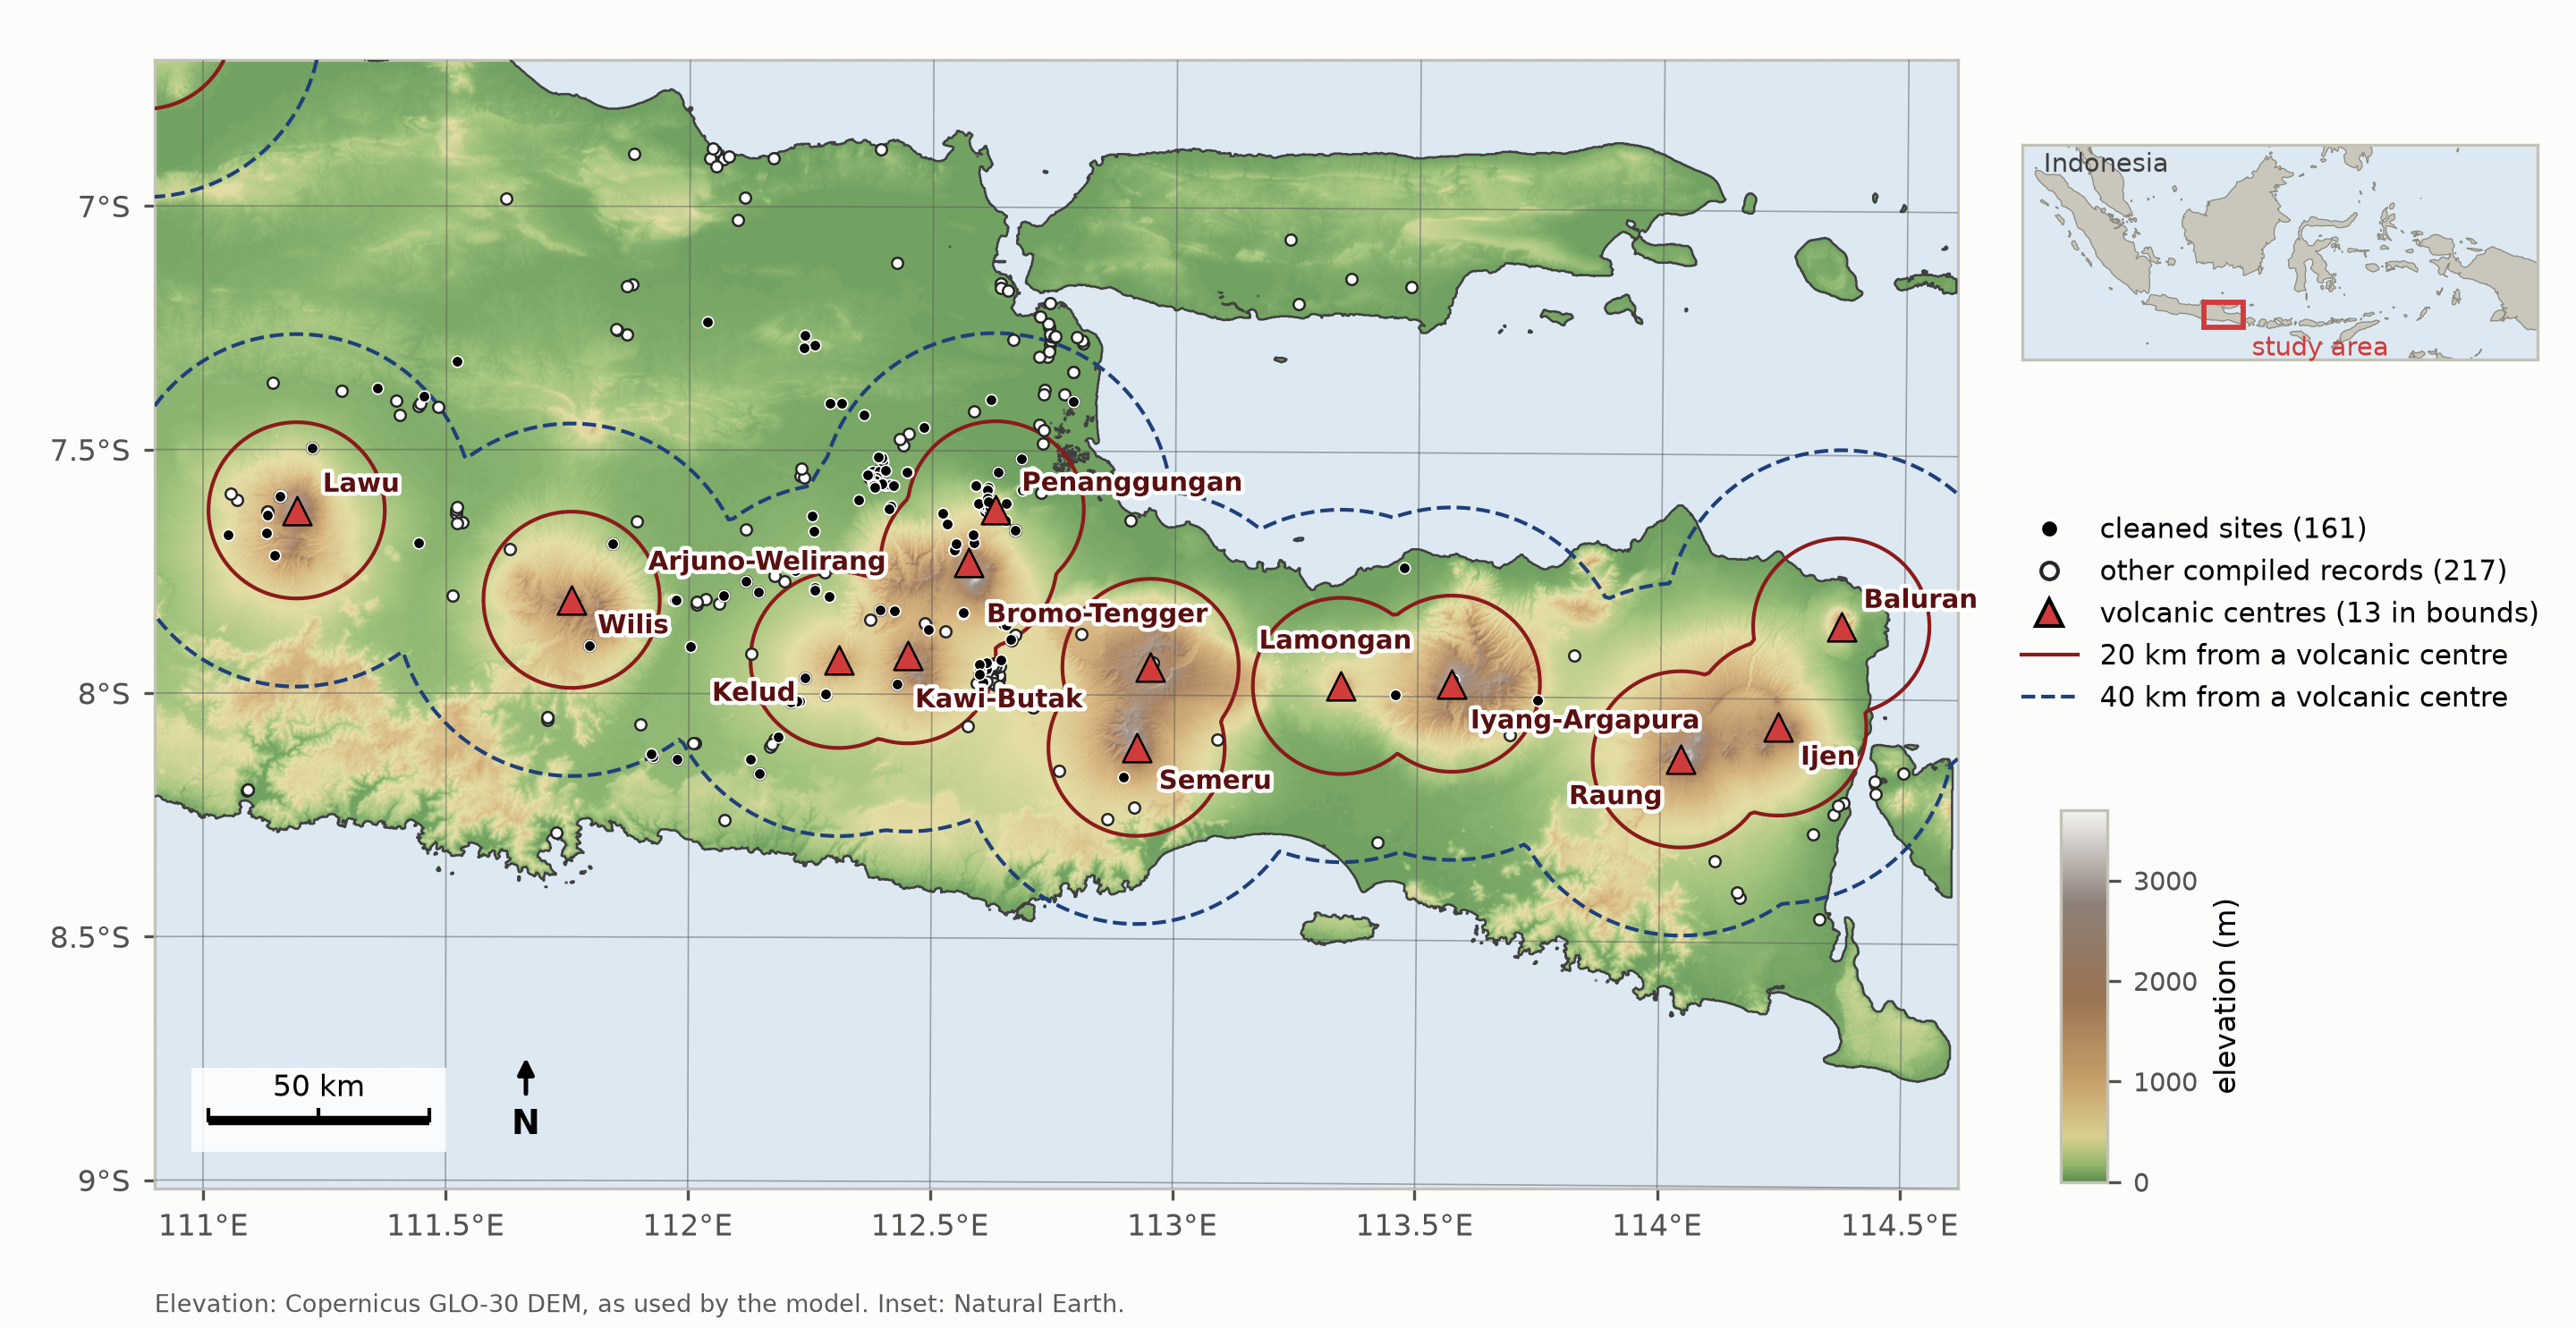
\includegraphics[width=\textwidth]{fig01_study_area_v03.png}
\caption{Study area in East Java, Indonesia, showing the 378 compiled presence records used for modelling (filled: the 161 sites of the cleaned subset, Section~\ref{sec:presence}; open: the other 217 records) and the 13 canonical volcanic centres inside the paper's stated bounds (111--115$^\circ$E), used as post-hoc diagnostics only.}
\label{fig:studyarea}
\end{figure}

% ============================================================================
\section{Materials and Methods}
% ============================================================================

\subsection{Data, covariates, and the principle of role separation}
\label{sec:covariates}

Usable presences after covariate filtering were 378 (111--115$^\circ$E); the soil-coverage subset used once in E009 was 259.
These 378 are compiled records rather than a site catalogue.
They come from OpenStreetMap (279 rows), lists in the Indonesian and English Wikipedia (85) and Wikidata (14), they hold 335 distinct coordinates, and about a third are not archaeological sites: 124 are modern monuments, statues or memorials, and 13 are misplaced or are not sites at all (Central Javanese temples carrying East Javanese coordinates, a Balinese temple placed near Surabaya, a waterfall).
Because that composition bears on every model fitted to the records, we define a cleaned subset and report the real-data contrasts on both.
The cleaning drops the 85 rows whose coordinates were geocoded from their names (all rows taken from the Wikipedia lists), 124 modern monuments, and 8 temples of other regions, tourist objects and modern institutions, and then keeps one row per coordinate (which removes no further rows); 161 sites remain (155 from OpenStreetMap, 6 from Wikidata).
The original ladder (E007--E013, Section~\ref{sec:ladder}) is the object under examination and stays trained on the 378 records; the contrasts of Section~\ref{sec:artefact} and Section~\ref{sec:presence} are reported on both sets.
Every variable plays one analytical role, and the roles must not be mixed, because mixing them makes a suitability score uninterpretable: a low score could mean the place was unsuitable, or unsurveyed, or not preserved, and the model cannot say which.
We therefore keep only the suitability block as predictors, express accessibility through the background design (Section~\ref{sec:fourroles}), and treat preservation and volcanic proximity as diagnostics applied to the output.
Table~\ref{tab:roles} assigns every variable a single role.

\begin{table}[h]
\centering
\resizebox{\textwidth}{!}{%
\begin{tabular}{llp{5.6cm}p{4.2cm}}
\toprule
Variable & Source & Analytical role & How it enters \\
\midrule
elevation & Copernicus GLO-30 DEM, 30 m, decimated $\times$10 ($\sim$300 m) & Suitability (terrain) & training feature \\
slope & derived from DEM & Suitability (terrain cost) & training feature \\
TWI & topographic wetness index, derived from DEM & Suitability (water availability) & training feature \\
TRI & terrain ruggedness index, derived from DEM & Suitability (terrain cost) & training feature \\
aspect & derived from DEM & Suitability (insolation/orientation) & training feature \\
river\_dist & OSM/HydroSHEDS, Euclidean distance & Suitability (water access); added at E008 & training feature \\
clay, silt & SoilGrids topsoil & Preservation / substrate & features in \textbf{E009 only}; dropped (lowered AUC) \\
road\_dist & OSM roads (expanded class set from E012) & Accessibility / survey effort & \textbf{never a training feature} \\
volcano\_dist & canonical inventory, 30 centres (13 in bounds) & Taphonomy / burial --- diagnostic only & \textbf{never a training feature} \\
\bottomrule
\end{tabular}}
\caption{Covariates and their analytical roles. Roles are exclusive by construction: a suitability variable answers \emph{would people have settled here?}; an accessibility variable answers \emph{would we have found it?}; a preservation variable answers \emph{would it still be there to find?}. TWI (topographic wetness index) quantifies the tendency of a cell to accumulate water; TRI (terrain ruggedness index) quantifies local elevation difference as a proxy for terrain cost.}
\label{tab:roles}
\end{table}

This separation is not a technicality.
It is central to this paper: the variable that defines the target-group background (accessibility, through \texttt{road\_dist}) is kept out of the features, so accessibility can affect the reported numbers only through the background design, which is what Section~3 examines.

\subsection{The modelling pipeline}
\label{sec:pipeline}

We model binary presence/background suitability.
The pseudo-absence (background) ratio is fixed at 1:5 throughout.
Three learners are compared: XGBoost \citep{chen2016} (primary), RandomForest \citep{breiman2001}, and a Maximum Entropy model \citep{phillips2006, elith2006}.
The Maximum Entropy model is the \texttt{elapid} implementation of maxnet, with linear, hinge and product features, regularisation multiplier $\beta = 1.5$ and a cloglog transform; $\beta$ is swept from $0.5$ to $4.0$ in Section~\ref{sec:artefact} to confirm the result is not an artefact of that setting.
Validation uses 5-fold deterministic spatial block cross-validation at a baseline block size of 0.45\textdegree{} ($\sim$50~km).
Primary metrics are AUC and the True Skill Statistic (TSS), the latter preferred to kappa because it does not vary with prevalence in the way kappa does \citep{allouche2006}.
Both are discrimination metrics computed against whatever background is supplied to them, which is precisely the property this paper is about \citep{lobo2008, guillera2015}.
The original pipeline set itself a target of spatial AUC $> 0.75$ under block cross-validation.

\subsection{The experiment progression, as the object under examination}
\label{sec:progression}

Seven iterative experiments (E007--E013) built the model whose evaluation we now examine.
They are the object of the analysis, not its result, so we summarise them in one table and two paragraphs and move the per-iteration detail to the supplement.
Table~\ref{tab:inclusion} states exactly which covariates each experiment used, read from the analysis scripts.

\begin{table}[h]
\centering
\resizebox{\textwidth}{!}{%
\begin{tabular}{lccccccccl}
\toprule
Exp. & elev & slope & twi & tri & aspect & river & road & Background design & Rep.\ spatial AUC \\
\midrule
E007 v1  & \cmark & \cmark & \cmark & \cmark & \cmark & --    & --    & uniform random, 1:5, 2 km buffer & 0.659 \\
E008 v2  & \cmark & \cmark & \cmark & \cmark & \cmark & \cmark & --    & uniform random, 1:5 & 0.695 \\
E009 v3  & \cmark & \cmark & \cmark & \cmark & \cmark & \cmark & --    & uniform random, 1:5 (+clay/silt) & 0.664 $\downarrow$ \\
E010 v4  & \cmark & \cmark & \cmark & \cmark & \cmark & \cmark & bg    & TGB (major road) & 0.711 \\
E011 v5  & \cmark & \cmark & \cmark & \cmark & \cmark & \cmark & bg    & TGB, parameters swept & 0.725 \\
E012 v6  & \cmark & \cmark & \cmark & \cmark & \cmark & \cmark & bg    & TGB, expanded road classes & 0.730 \\
E013 v7  & \cmark & \cmark & \cmark & \cmark & \cmark & \cmark & bg    & hybrid = TGB pool + regional blend + hard negatives & 0.768 best / 0.751 seed-avg \\
\bottomrule
\end{tabular}}
\caption{Per-experiment covariate inclusion. \cmark\ = training feature; -- = not used; \emph{bg} = used to construct the background, never as a feature. Reproducibility: rasters in \texttt{data/processed/dem/}, presences in \texttt{data/processed/east\_java\_sites.geojson} (378 valid in bounds), deterministic 5-fold spatial blocking at 0.45\textdegree{}, pseudo-absence ratio 1:5 throughout. E010--E013 use \texttt{road\_dist} to build the background while excluding it from the features.}
\label{tab:inclusion}
\end{table}

Two paragraphs of interpretation.
Feature-only expansion plateaued (E007--E009): adding river distance helped ($+0.036$) and adding soil covariates hurt ($-0.031$).
Background redesign then delivered the monotone rise (E010--E013) that we initially read as evidence that pseudo-absence realism dominates feature accumulation.
The remainder of this paper asks whether that rise is real.

The hybrid design of E013 blends a TGB candidate pool with a regional quota and a fraction of `hard negatives', sweeping \texttt{region\_blend} $\in \{0.0,0.3,0.5,0.7\}$ and \texttt{hard\_frac} $\in \{0.0,0.15,0.30\}$.
% PI prose 2026-10-22 (written in Indonesian, translated by Claude; log: PI_PROSE_LOG_R2.md, passage 7; ledger C080).
In this study, hard negatives are defined as points at a standardised environmental distance ($z$) of 2--5 from the mean site environment (Table~\ref{tab:keyterms}); although the targeted proportion in the hybrid design is 30\%, the realised proportion reached 0.62.
This happens because the remaining 70\% of points are drawn from a background pool in which about half of the members already have $z \geq 2$, not because of a particular bias of the TGB, whose proportion of such points (0.485) is close to that of the random background (0.503).
This pool-composition effect bears on the absolute AUC values and is part of why a common evaluation background matters (Section~\ref{sec:artefact}).

\subsection{The four roles of \texttt{road\_dist}}
\label{sec:fourroles}

\texttt{road\_dist} is deliberately never a training feature, yet it does four jobs at once: it (i) defines the TGB acceptance probability, (ii) defines the hybrid background pool, (iii) defines the accessibility-proxy holdout split (E014, Section~\ref{sec:holdout}), and (iv) serves as a visibility proxy in the diagnostic suite.
% PI prose 2026-10-22 (passage 8B).
The original pipeline included diagnostic tests, named Test 1 and Test 3 in its code. In Test 1, the correlation between predicted suitability and the distances to volcanoes, to roads and to the nearest site is examined; the diagnostic is considered failed only if the absolute Spearman correlation exceeds 0.5.
Test 3 compared model performance across road-distance quartiles; it was scored on the design's own background, so its result is subject to the artefact this paper describes and is not used here. The volcano-related component of Test 1 is reported in Section~\ref{sec:diagnostics}.
Because the variable used to build the background can also affect the reported metric values, the role of \texttt{road\_dist} in building the background and in the diagnostics needs to be explained here, in the Methods, together with the other covariates.
This is also what makes the approach specifically archaeological: the archaeological content is not in the label set, it is in the background design: a claim about where a survey could plausibly have detected a site had one been present.

\subsection{The accessibility-proxy holdout (E014)}
\label{sec:holdout}

% PI prose 2026-10-22 (passage 8C).
E014 is an \emph{accessibility-proxy holdout}: the model is trained on sites $\leq 1$~km from a road and tested on sites $>1$~km away, with road accessibility standing in for discovery order (sites far from roads stand in for sites found late), so the split reflects differences in accessibility, not differences in time.
The model yields an AUC of 0.755.

\subsection{The refutation design: E217--E224}
\label{sec:refutation}

The eight experiments E217--E224 are the paper's centrepiece. E218 and E220--E224 were run from written designs with decision rules; only for E224 was the design committed to the public repository before the run (for the others, design and results were committed together), and E217 and E219 have no written design.

One deviation from the original pipeline must be stated before the results, because it bears on how they should be read.
E217--E224 draw background points from a decimated raster lattice ($\sim$300~m spacing) rather than by the continuous-coordinate rejection sampling used in E007--E013.
This was a deliberate choice: it gives every background design a single shared sampling frame, which is a precondition for the common-background comparison, and it keeps a factorial benchmark tractable.
The cost is that absolute AUCs in E217--E224 are not directly comparable to the original E007--E013 values.
The quantities we interpret are therefore \emph{within-benchmark contrasts} (design against design, and own-background against common-background, under identical folds), not the absolute levels.
Because the lattice is a departure from the original pipeline, E218 re-ran the comparison at half that spacing ($\sim$150~m, 5 seeds): the ladder persists on own backgrounds (random $0.711 \rightarrow$ hybrid $0.757$) and stays flat on the common background (random $0.705 \rightarrow$ hybrid $0.704$), so the conclusion does not depend on the lattice.

\paragraph{E217 -- common-background benchmark.}
MaxEnt, XGBoost and RandomForest are run under \emph{identical} spatial-block folds and \emph{identical} background designs as E007--E013, but each design is scored against a \emph{common} evaluation background shared across designs, so that the comparison is identified.
A second feature set (\texttt{terrain} alone, 5 vars vs \texttt{terrain\_river}, 6 vars) lets us compare a feature effect against a background-design effect.

\paragraph{E218 -- the evaluation artefact, isolated.}
Three training designs are each scored against four evaluation backgrounds (own + three foreign), exposing how much of each design's apparent lead comes from being scored on its own background.

\paragraph{E220 -- does the selection criterion have an interior optimum?}
We vary the share of hard negatives in the background from 0 to 1 and ask whether the AUC-on-own-background criterion ever tells a researcher to stop before the end of that range.

\paragraph{E221 -- seed stability of the priority map.}
Across random seeds, how much of the top-decile priority map turns over, and how much does averaging seeds reduce it?

\paragraph{E222 -- synthetic ground truth.}
Four synthetic worlds of known intensity surface let us compare \emph{reported} AUC (own-background) against \emph{true} recovery (common-background) where ground truth is not in question.

\paragraph{E223 -- confidence intervals and regularisation.}
Bootstrap and equivalence CIs bound the ladder gain; a MaxEnt regularisation sweep ($\beta = 0.5$--$4.0$) tests whether the artefact is an overfit of an unregularised model.

\paragraph{E224 -- testing one explanation of the TGB null (Section~\ref{sec:tgbnull}).}
We proposed that the TGB null in E222 was structural, tested it, and the test failed; the null is reported as unexplained.

% ============================================================================
\section{Results}
% ============================================================================

\subsection{The reported ladder}
\label{sec:ladder}

The seven experiments (E007--E013) show the AUC rising from 0.659 under a random background (E007) to a 20-seed average of 0.751 under the hybrid design (E013).
That rise of 0.092 runs through the addition of environmental features, the introduction of target-group background (TGB), and the combination of several background-selection strategies.
For E013 the seed-averaged AUC and TSS are $0.751 \pm 0.013$ and $0.465 \pm 0.021$ respectively.
At first sight, this supports the reading that increasingly realistic background designs improve model performance.
That reading still needs testing: the null models in Table~\ref{tab:nullmodel} are evaluated on a different background, and E013 is scored on its own.
DKNS also uses the actual site locations, so it is not a fully fair comparison.

\begin{table}[h]
\centering
\resizebox{\textwidth}{!}{%
\begin{tabular}{llccccccc}
\toprule
Exp. & Pseudo-absence strategy & XGB AUC & RF AUC & Best AUC & XGB TSS & RF TSS & Status \\
\midrule
E007 & Random                 & 0.659 $\pm$ 0.077 & 0.656 $\pm$ 0.090 & 0.659 & 0.318 $\pm$ 0.126 & 0.314 $\pm$ 0.133 & REVISIT \\
E008 & Random + river feature & 0.685 $\pm$ 0.074 & 0.695 $\pm$ 0.107 & 0.695 & 0.345 $\pm$ 0.135 & 0.379 $\pm$ 0.200 & REVISIT \\
E009 & Random + soil features & 0.664 $\pm$ 0.049 & 0.643 $\pm$ 0.054 & 0.664 & 0.337 $\pm$ 0.083 & 0.312 $\pm$ 0.072 & REVISIT \\
E010 & TGB (major road)       & 0.711 $\pm$ 0.085 & 0.699 $\pm$ 0.081 & 0.711 & 0.384 $\pm$ 0.150 & 0.380 $\pm$ 0.130 & REVISIT \\
E011 & TGB tuned              & 0.725 $\pm$ 0.084 & 0.716 $\pm$ 0.081 & 0.725 & 0.447 $\pm$ 0.184 & 0.408 $\pm$ 0.147 & REVISIT \\
E012 & TGB tuned (expanded)   & 0.730 $\pm$ 0.085 & 0.724 $\pm$ 0.081 & 0.730 & 0.420 $\pm$ 0.170 & 0.413 $\pm$ 0.152 & REVISIT \\
E013 & Hybrid bias-corrected  & 0.768 $\pm$ 0.069 & 0.742 $\pm$ 0.070 & 0.768 & 0.507 $\pm$ 0.167 & 0.458 $\pm$ 0.126 & SUCCESS \\
\bottomrule
\end{tabular}}
\caption{Experiment progression E007--E013 (the ladder under examination).}
\label{tab:progression}
\end{table}

\begin{figure}[h]
\centering
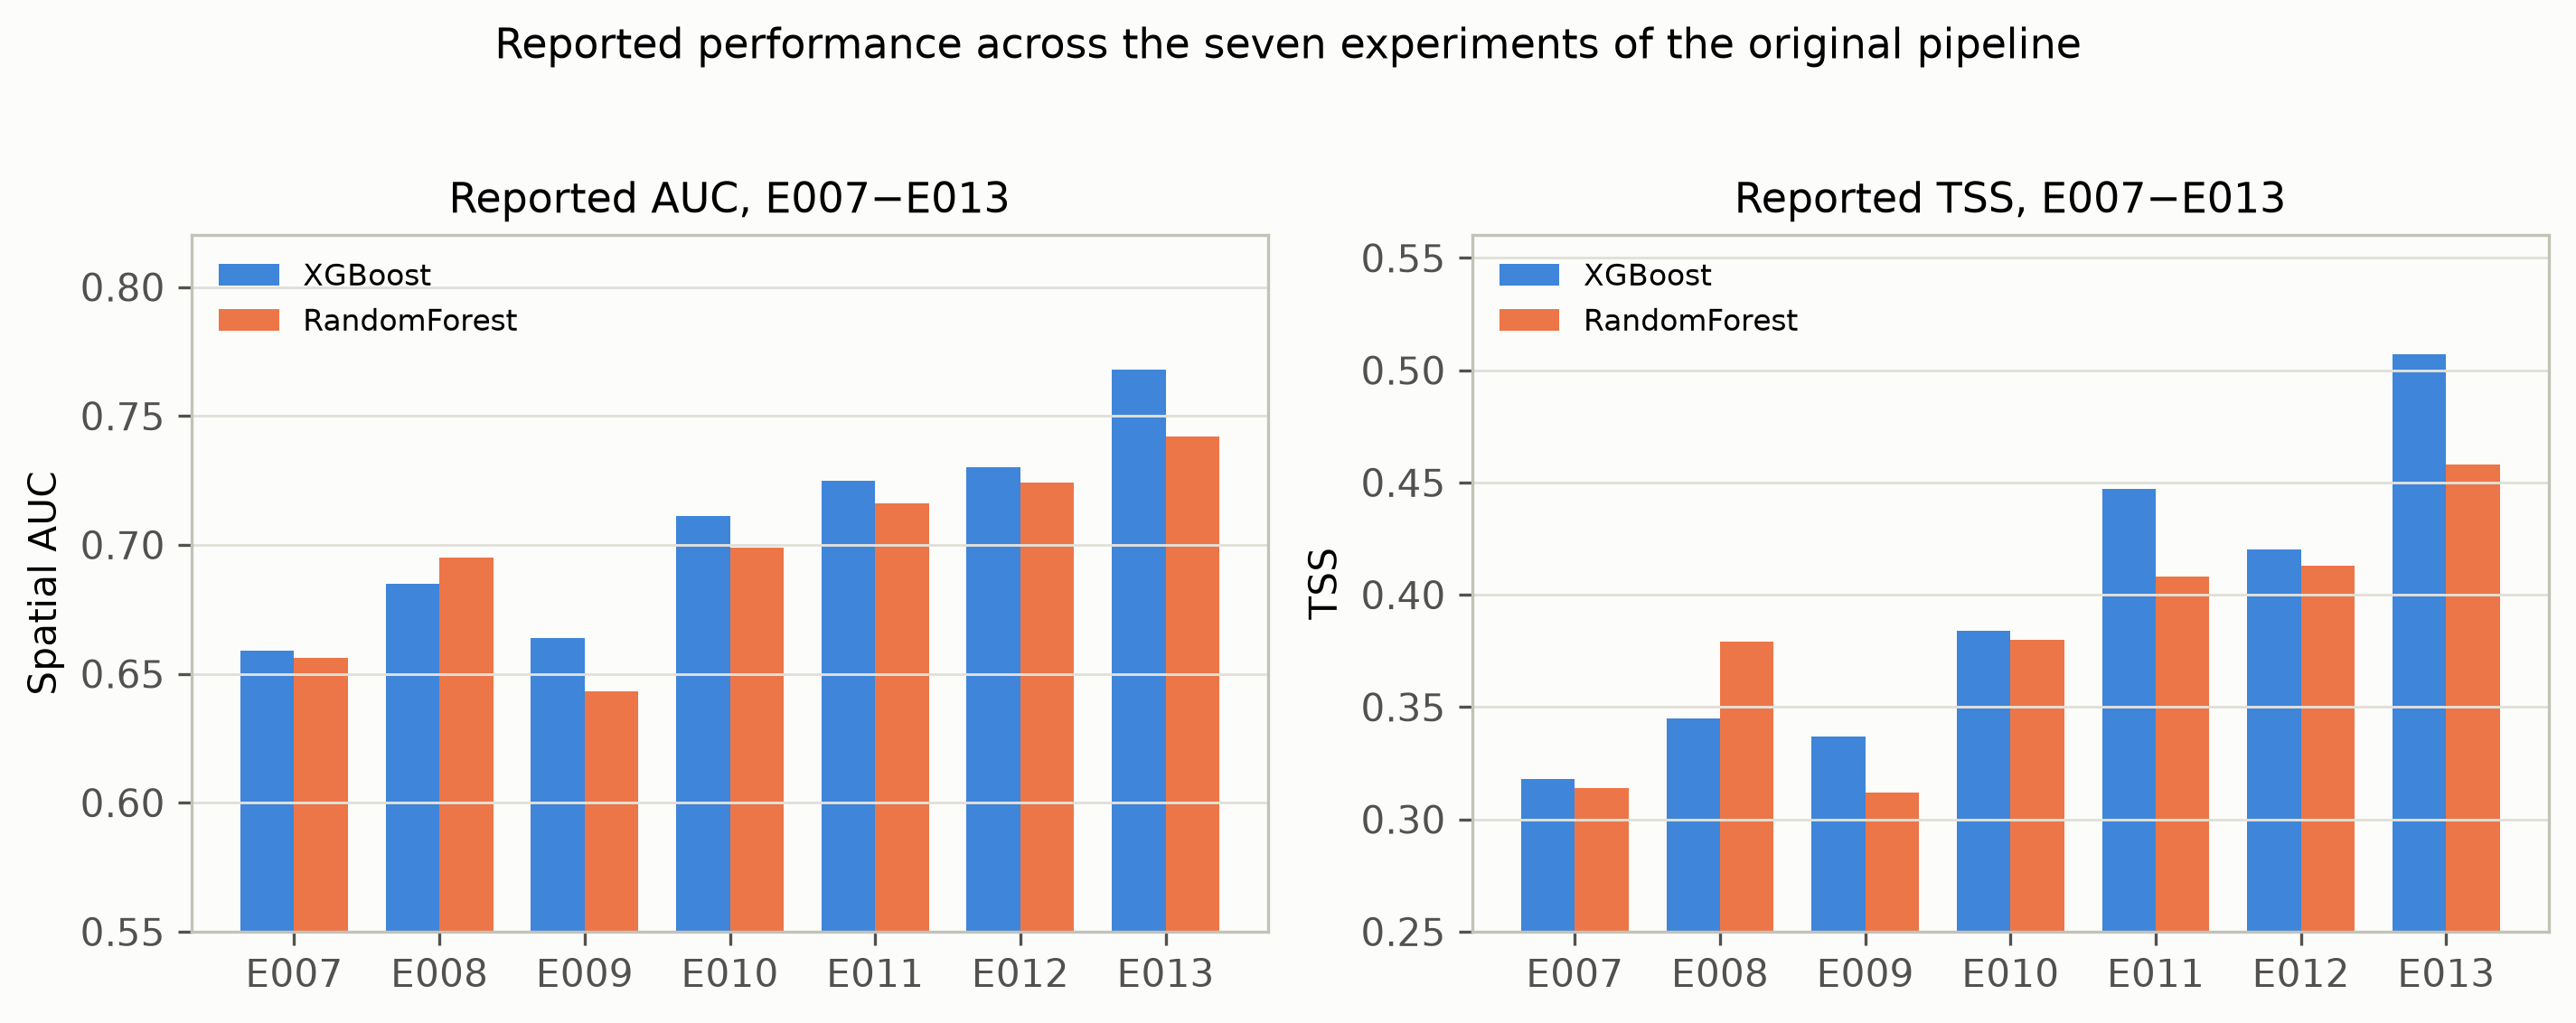
\includegraphics[width=0.95\textwidth]{fig02_progression_v03.png}
\caption{Reported AUC and TSS across the seven experiments of the original pipeline (E007--E013; Table~\ref{tab:progression}). This is the ladder under examination; Section~\ref{sec:artefact} asks whether the rise \emph{between} E007 and E013 is real.}
\label{fig:progression}
\end{figure}

\begin{table}[h]
\centering
\small
\begin{tabular}{lccc}
\toprule
Model & AUC & Std & Gap vs E013 \\
\midrule
Random (chance)              & 0.500 & 0.000 & $+$0.251 \\
Heuristic (river $<$ 2 km)   & 0.581 & 0.054 & $+$0.170 \\
DKNS (spatial interpolation) & 0.646 & 0.032 & $+$0.105 \\
\textbf{E013 XGB (seed-avg)} & \textbf{0.751} & 0.013 & --- \\
E013 XGB (best run)          & 0.768 & 0.069 & --- \\
\bottomrule
\end{tabular}
\caption{Null-model comparison under spatial CV. Gaps are computed against the E013 seed-average (0.751), not the best run, because a single run is not a reportable quantity (Section~\ref{sec:prioritymaps}). The nulls are scored on a regular grid of all cells, while the E013 column is the model's own-background seed-average --- so the margins shown still mix evaluation backgrounds, a defect corrected in Section~\ref{sec:artefact}, where the consequence for this level comparison is stated. DKNS (distance to known nearest site) uses site locations as an unfair upper bound.}
\label{tab:nullmodel}
\end{table}

\subsection{The ladder does not survive a common evaluation background}
\label{sec:artefact}

To test whether the AUC rise in the preceding experiments reflects a real gain in model skill, every design was re-scored on the same evaluation background.
The test uses three algorithms --- XGBoost, Random Forest and Maximum Entropy (MaxEnt) --- with five seeds and the same spatial-block cross-validation split.
This allows a fairer comparison, because every model is scored on an identical set of background points rather than on the background its own design produced.
On the 378 compiled records with the full feature set, the decomposition gives the background redesign a contribution of only $-0.0142$ AUC, with a seed-cluster interval of $-0.021$ to $-0.005$.
Only 3 of the 15 seed$\times$algorithm combinations are positive.
With terrain features alone, the same redesign contributes $+0.0054$.
Adding distance to rivers has a more consistent effect: $+0.0424$ AUC, positive in all 12 paired comparisons.
On the compiled data, then, the gain tracks the added environmental information (distance to rivers) more than the change in background design.

The next test compares the hybrid design with the random design under several kinds of evaluation background.
Hybrid scores higher than random on all three algorithms when both are evaluated on the hybrid background.
The advantage disappears when the evaluation uses the uniform, TGB or stratified background: on each of those three, not one of the three algorithms shows it.
Scored on its own background instead, the redesign contributes $+0.0316$ on average: $+0.0145$ for MaxEnt, $+0.0431$ for XGBoost and $+0.0373$ for Random Forest.

The size of that effect is clearest in the test aimed at the hybrid design.
On the 378 compiled records, own background minus uniform background is positive in all 60 seed$\times$algorithm combinations.
The mean inflation is $+0.037$ AUC, over a range of $+0.005$ to $+0.084$.
That is the same order of magnitude as the ladder rise of $+0.092$.
The effect is not uniform across designs, however.
For TGB, scoring on the own background instead gives an AUC $0.0054$ lower on average than the uniform background, with only 22 of 60 combinations positive.
TGB against the random design on the own background differs by only $+0.003$.
The rise at the TGB step (E010--E012) therefore cannot be explained as own-background inflation.
That result does not recur in the benchmark, but that is not evidence enough to call the TGB step an evaluation artefact.
It has to be kept distinct from the effect identified directly on the hybrid design.

To test whether the same tendency appears where the truth is known, we ran an experiment on synthetic data with a prescribed intensity surface.
Here the reported AUC --- own background --- is compared with how well the model recovers the true pattern when scored on the common background.
For the hybrid design the reported AUC exceeds the true performance in all 240 runs, with a median gap of $+0.238$.
For the random design it happens in 52 of 60 runs (median $+0.020$), and for TGB in 51 of 60 (median $+0.014$).
Across both surfaces, 343 of 360 runs put the reported AUC above the true performance.
In the random and TGB designs, however, part of the gap comes from the difference between the observed presence sample and the full true presences, not from the background choice alone.
The synthetic experiment therefore strengthens the evidence that scoring a design on its own background --- the hybrid design above all --- can overstate performance (Figure~\ref{fig:artefact}).

That evidence was then checked by statistical tests and a sensitivity analysis.
Equivalence confidence intervals reject $+0.092$ in all 12 algorithm$\times$evaluation-background combinations.
A presence-block bootstrap was run for 30 replicates; one was discarded for having fewer than 50 out-of-bag sites, leaving 29.
The upper confidence bounds are $+0.008$ for MaxEnt, $+0.025$ for XGBoost and $+0.026$ for Random Forest, all well below the $+0.092$ rise.
The bootstrap is small, but it still rejects the rise: the distance between the bounds and the value under test is wide.
It does not mean the interval end-points are estimated with high precision.
Varying the MaxEnt regularisation over $\beta = 0.5$--$4.0$ gives contributions of $-0.020$ to $-0.022$, with one of ten runs positive.
The finding is not an artefact of an under-regularised or overfitted model.

The same finding changes how Table~\ref{tab:nullmodel} should be read.
In the earlier comparison E013 has a seed-averaged AUC of $0.751$, while the nulls are scored on a regular grid covering every cell of the study area.
Since the two groups are scored on different backgrounds, the $+0.105$ margin over the spatial-interpolation null DKNS (AUC $0.646$) is potentially too high.
Scored on the common uniform background, the XGBoost design of E013 falls to $0.706$.
It stays above DKNS, but the margin shrinks to about $+0.06$.
The worst-seed margin, $+0.083$, is likewise close to the detection floor of $+0.03$ discussed in Section~\ref{sec:ci}.
The $0.751$ comes from the original pipeline and the $0.706$ from the lattice-based benchmark, so the two do not share an identical sampling procedure; the shrinkage is best read as an order of magnitude, not as the direct difference between two fully comparable measurements.
What survives is that environmental features capture structure beyond interpolation from the nearest site.
What does not survive is the size of the advantage once the evaluation background is made uniform.
Table~\ref{tab:nullmodel} is therefore an upper bound on the advantage over the nulls, not a lower bound that can be relied on.

\begin{figure}[h]
\centering
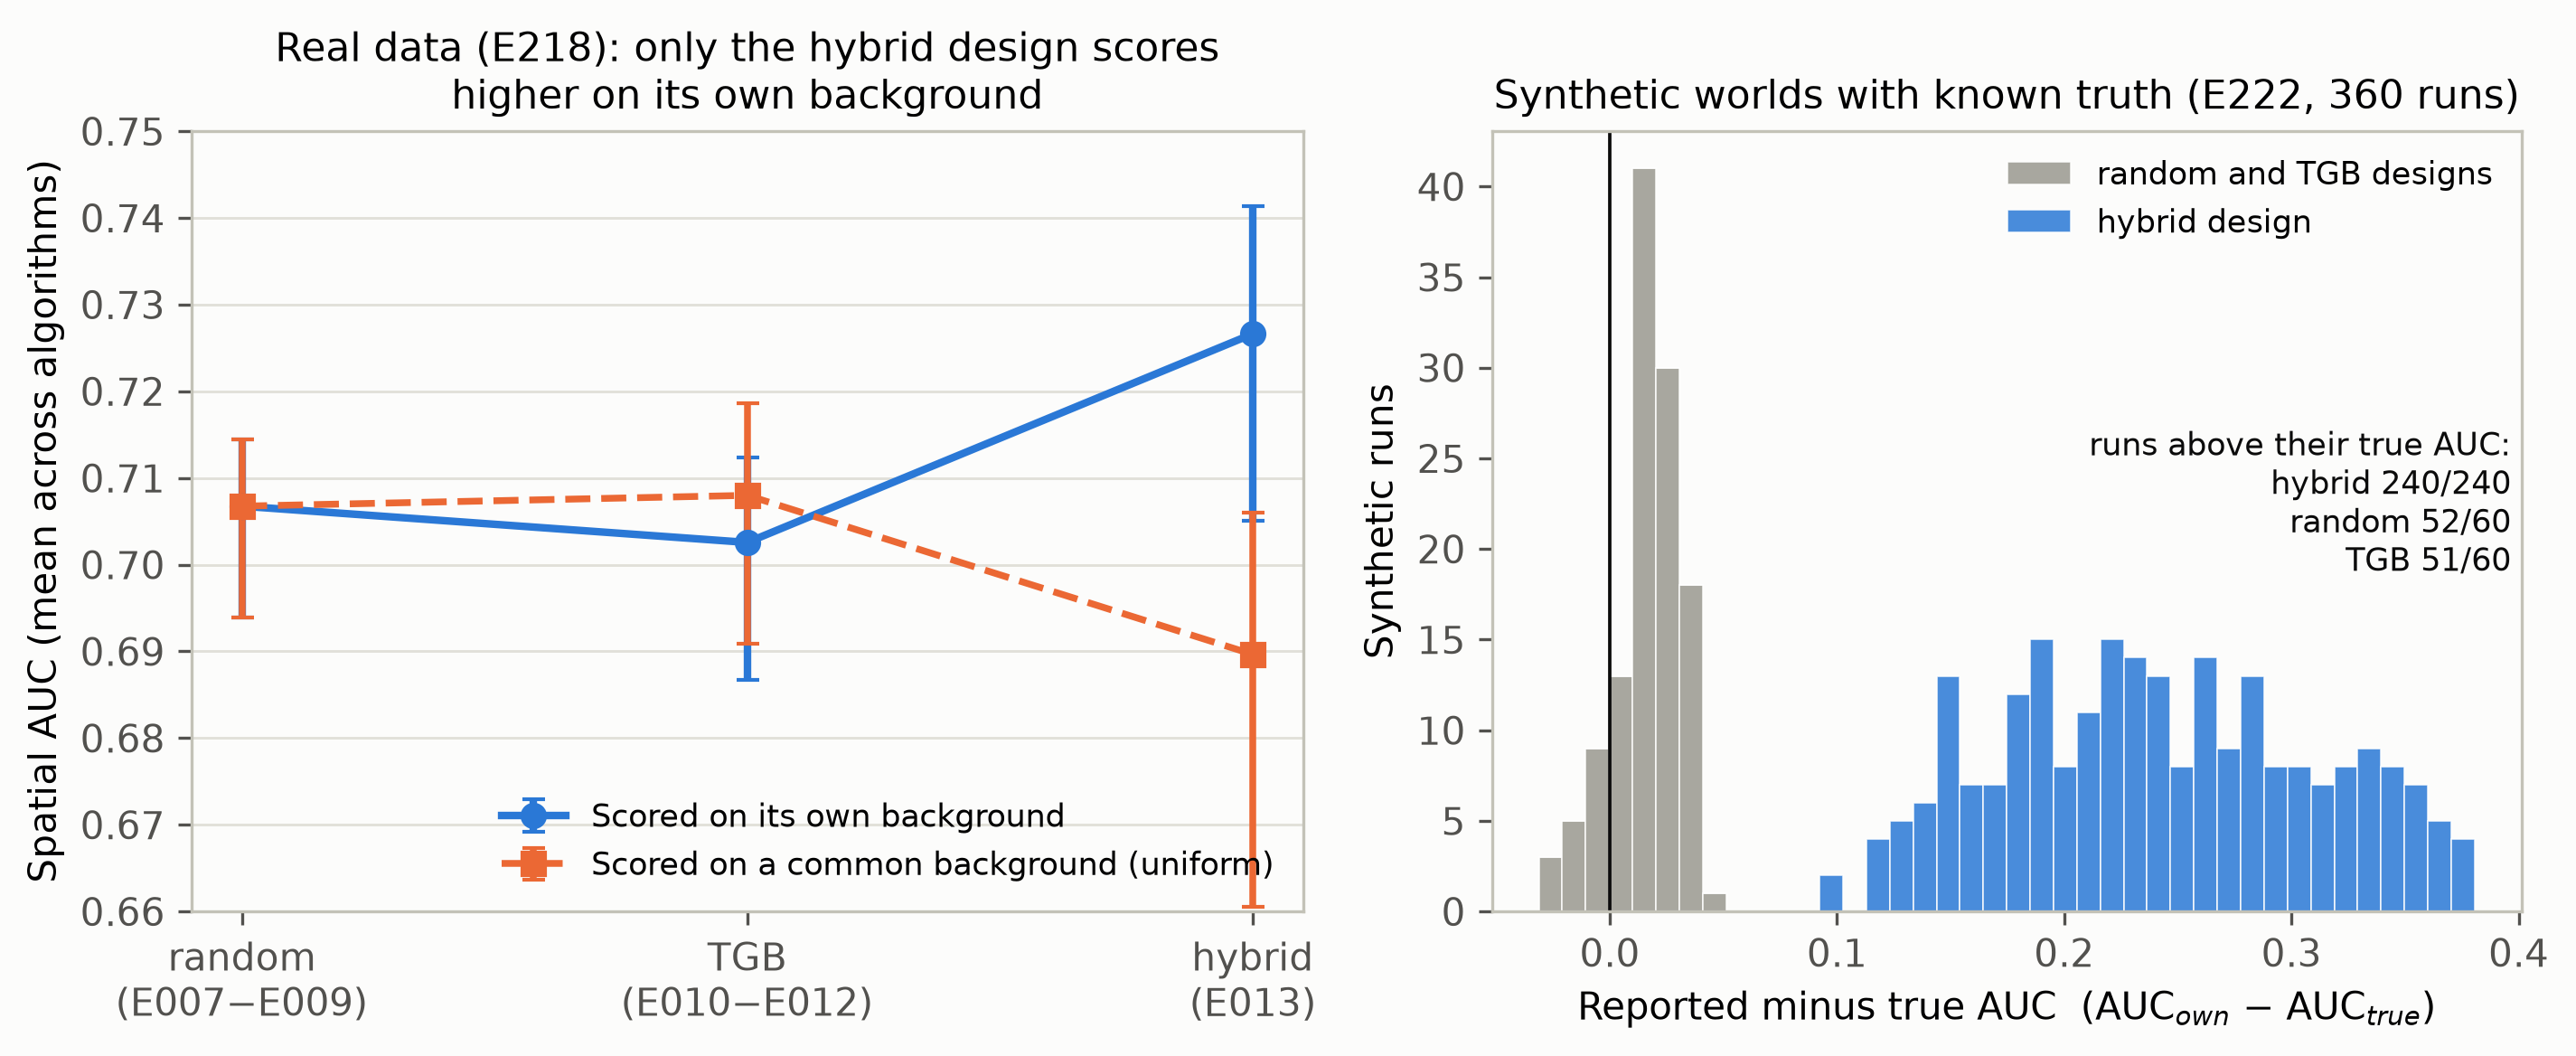
\includegraphics[width=\textwidth]{fig03_artefact_v03.png}
\caption{The evaluation artefact. Left: reported AUC (evaluated on a design's own background) against the same designs held to a common background (uniform). Only the hybrid design scores higher on its own background. Right: reported minus true AUC in 360 synthetic runs of known ground truth, by design (hybrid 240/240 runs positive; random 52/60; TGB 51/60).}
\label{fig:artefact}
\end{figure}

\subsection{The presence records and a cleaned subset}
\label{sec:presence}

The presence data consist of 378 records at 335 distinct coordinates, compiled from public sources rather than from a verified site catalogue.
Not every record is an archaeological site: 124 are modern monuments, statues or memorials, and 8 more are temples from other regions, tourist objects or modern institutions.
About a third of the set therefore carries a defect that could affect the modelling results.
Every analysis was therefore repeated on a cleaned subset (E236): the 85 records geocoded from a name in a Wikipedia list, the 124 modern monuments and the 8 other non-site records were removed, leaving 161 sites (155 from OpenStreetMap, 6 from Wikidata).
Every script was kept unchanged apart from the presence file it reads, so the two sets differ only in their presences; Table~S9 reports every quantity for both.

On the cleaned sites the contrast that is null on the compiled records becomes positive: with a common evaluation background, the redesign contributes $+0.0507$ over five seeds and $+0.0510$ [$+0.039$, $+0.063$] over ten, positive in 29 of 30 seed$\times$algorithm cells and for each algorithm separately (XGBoost $+0.038$, Random Forest $+0.044$, MaxEnt $+0.072$).
Two disjoint five-seed ensembles give $+0.0505$ and $+0.0516$.
Scored on its own background the same contrast reaches $+0.098$, so own-background evaluation overstates the gain by $+0.047$ --- close to the size of the gain itself.

Own-background inflation survives the change of data: hybrid is reported higher on its own background than on the uniform one in 54 of 60 cells (mean $+0.041$), against 60 of 60 (mean $+0.037$) on the compiled records.
The TGB step is likewise absent in both sets (TGB minus random $-0.005$ on the own background and $+0.001$ on the common one).
Two differences remain.
On the clean subset hybrid beats random under every evaluation background --- uniform, TGB, hybrid and stratified --- for all three algorithms; on the compiled records, only on its own.
The hybrid advantage therefore depends on the quality of the presence data, while its inflation does not.

The selection criterion fails in the same way.
Raising the hard-negative share from $0.0$ to $1.0$ lifts the own-background AUC from $0.697$ to $0.866$, with the maximum at the end of the range tested, while the common-background AUC at shares of $0.0$, $0.3$ and $1.0$ is $0.680$, $0.713$ and $0.656$.
The configuration with the highest own-background AUC therefore has the lowest common-background score: on this set the criterion does not merely fail to stop, it steers the choice away from the best setting.

Priority maps remain unstable.
Robust-core to contingent-fringe density ratios are $2.54$, $8.51$ and $5.30$ (Random Forest, XGBoost and MaxEnt); the top decile turns over by $41.6$--$54.8$~\% between seed pairs; two disjoint five-seed ensembles agree at a Jaccard overlap of $0.70$--$0.77$, against $0.76$--$0.86$ on the compiled records.
The fringe holds only 5, 15 and 5 sites, so the ratios indicate a direction rather than a precise size.

The elevation control points the same way in both sets.
Below 1,000~m the near $-$ far suitability difference is $+0.046$ for the random and TGB designs and $+0.060$ for the hybrid, against $+0.049$, $+0.049$ and $+0.060$ on the compiled records; only the hybrid meets the pre-registered SPECIFIC criterion, the summary across the three designs is inconclusive, and the two sensitivity definitions exchange their labels between the sets.
Cleaning the data therefore neither removes the elevation pattern nor makes it strong enough to support a general conclusion.
The section's summary stands: the redesign can deliver a real gain, but its size can still be overstated by own-background evaluation.

\subsection{The selection criterion has no interior optimum}
\label{sec:nooptimum}

The selection criterion is the AUC computed on a design's own background.
In the synthetic worlds it rises from $0.7367$ at a hard-negative share of $0.0$ to $0.8904$ at $1.0$.
On the real data it moves from $0.7208$ to $0.8435$ across the eleven points tested, with one dip of $0.0071$ between $0.0$ and $0.1$ and a continuous rise after it.
In both kinds of data, then, the maximum lies at the end of the range tested, not inside it (Figure~\ref{fig:dial}).
The criterion gives no indication of when to stop adding hard negatives.

The practical consequence is still small on the E013 grid, which covers only the shares $0.0$, $0.15$ and $0.30$.
The selection cost is computed as the AUC of the best design minus the AUC of the design selected by the criterion, on the same grid.
For the synthetic data the calculation uses the true AUC, whereas for the real data it uses the AUC on the common background, because the true AUC is not known.
The selection cost on that grid is $+0.0044$ on the real data; over 60 synthetic cases the median is $+0.0000$, the mean $+0.0012$ and the maximum $+0.0088$.
E013 stopped at $0.30$ because its grid ended there, not because the criterion marked that point as the place to stop.
The risk becomes much larger if the range is extended to $1.0$: the cost reaches $+0.0973$ on the real data and a median of $+0.1937$ on the synthetic data, positive in 60/60 cases.
The criterion selects the hybrid design at a share of $1.0$ in 60/60 synthetic cases, but in no case (0/60) is that the design with the lowest true AUC.
The problem, then, is not that the criterion always selects the worst design, but that it provides no mechanism to signal a stop.

\begin{figure}[h]
\centering
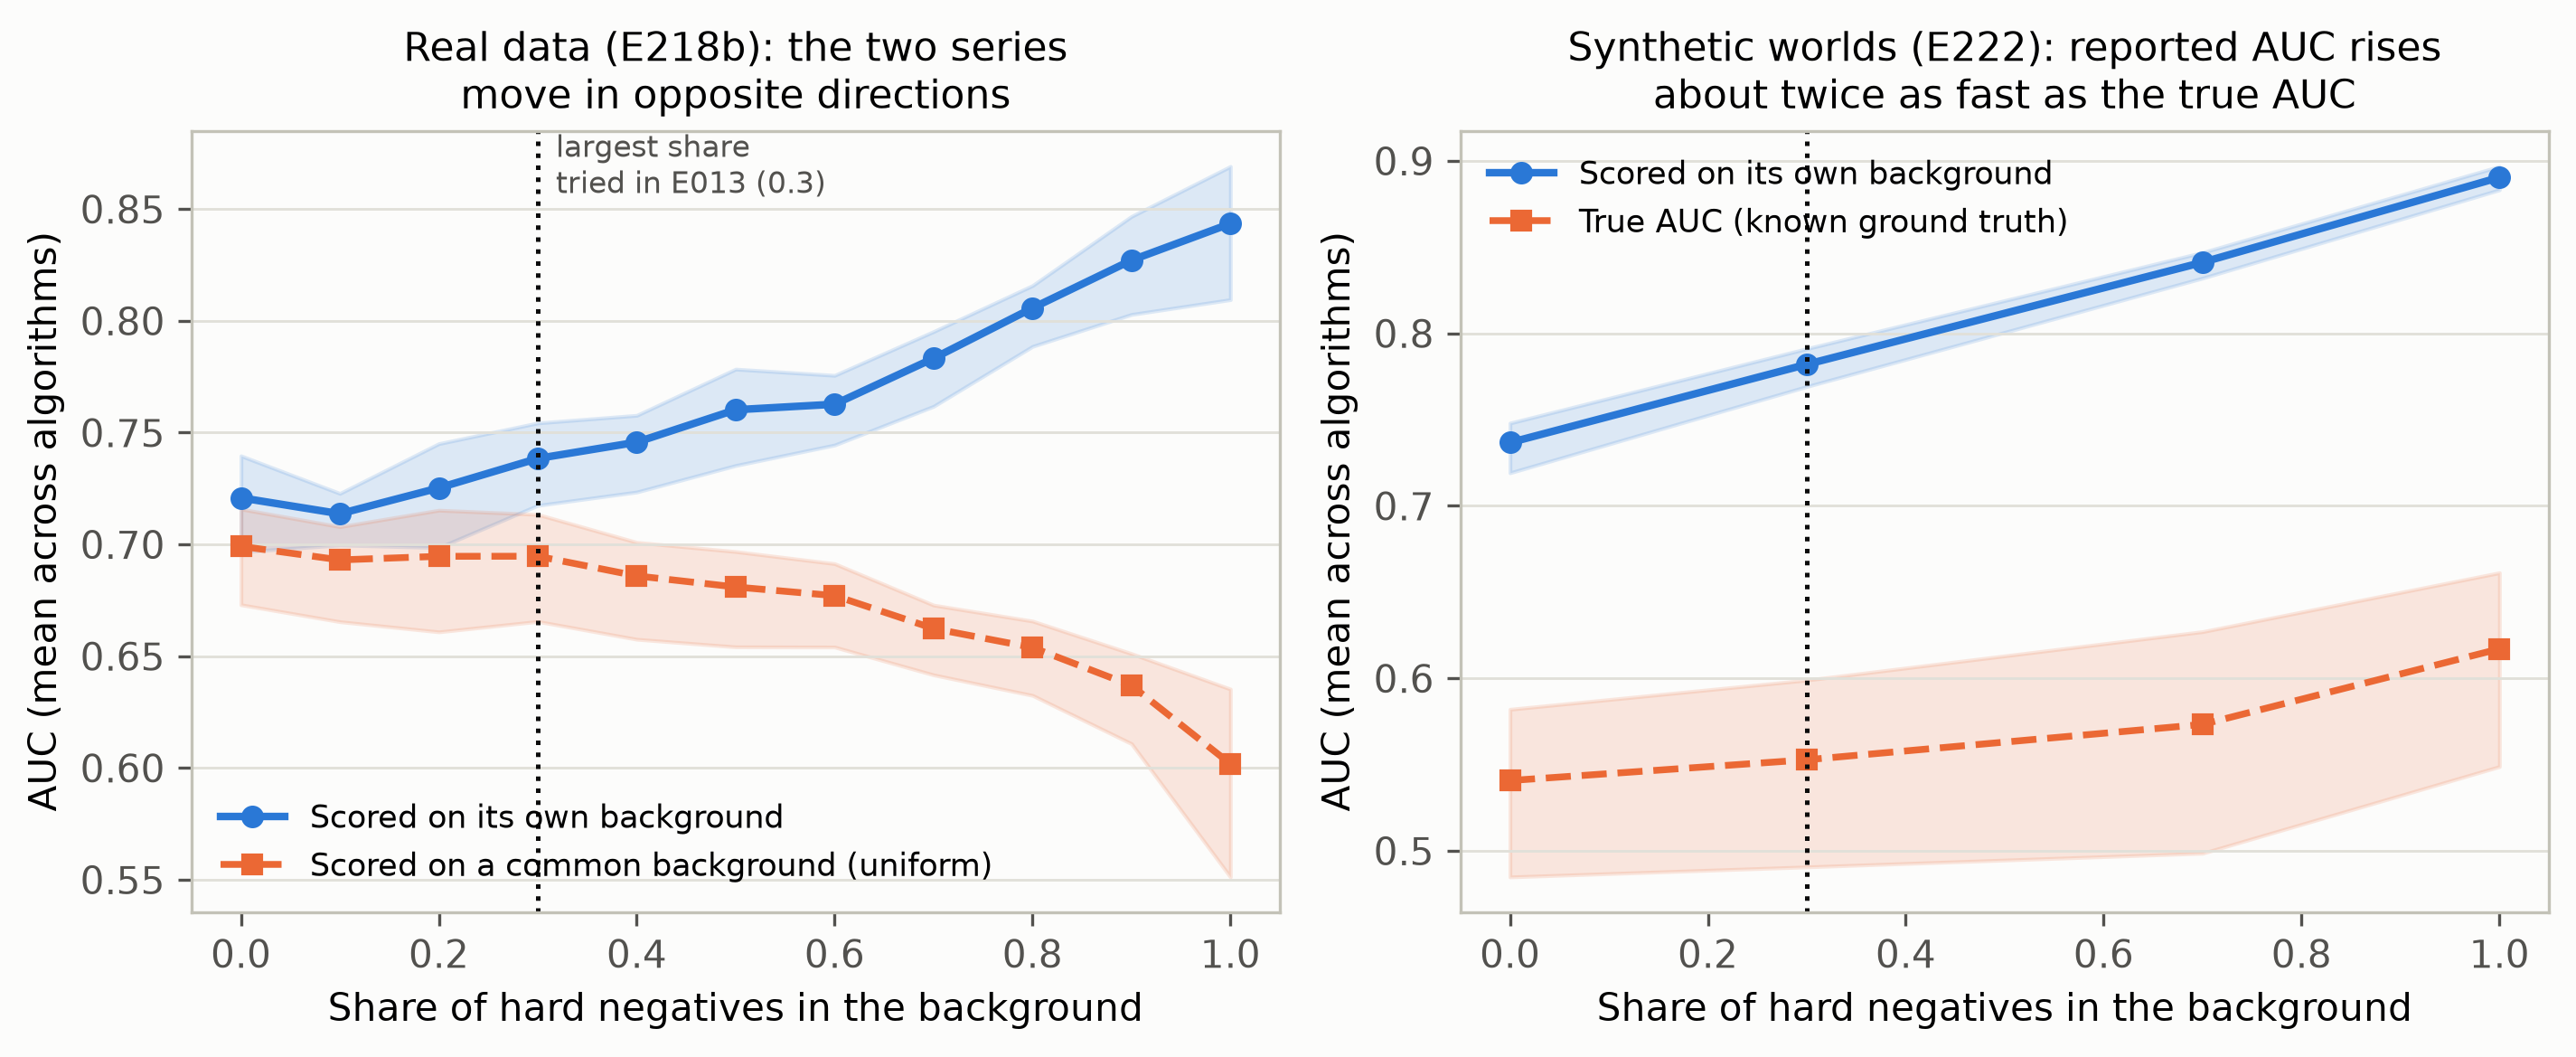
\includegraphics[width=\textwidth]{fig04_criterion_v03.png}
\caption{The selection criterion on a design's own background (solid) keeps rising to the end of the hard-negative range; the comparison series (dashed) falls on real data and rises only about half as fast on synthetic data, so the criterion has no interior optimum. Left: real data, scored on a common background; the two series move in opposite directions. Right: synthetic ground truth; reported performance moves about twice as fast as true performance. The dotted vertical line marks 0.30, the largest share tried in E013; the range tried here ends at $1.0$.}
\label{fig:dial}
\end{figure}

\subsection{The difference between reported and true AUC}
\label{sec:diverge}

In the synthetic worlds, raising the hard-negative share from $0.0$ to $1.0$ makes the AUC computed on each design's own background rise by $0.1538$.
The true AUC, however, rises by only $0.0764$, or roughly half as much.
On the real data the pattern is the opposite: the reported AUC rises by $0.1227$, while the common-background AUC falls by $0.0973$.
E222's written prediction that AUC inflation would increase with the share was not met.
In a single Spearman test pooled over all 240 hybrid runs, the value is only $\rho = 0.4395$: positive, but below the threshold of $0.5$.

\subsection{TGB shows no consistent advantage}
\label{sec:tgbnull}

Across the four synthetic regimes tested, TGB gives no consistent advantage over the random design.
For Worlds A and B combined, the TGB $-$ random difference in top-decile map agreement (Jaccard) is $-0.010$; TGB scores higher in 28/60 pairs (46.7\%), still below the specified threshold of 60\%.
The results also differ by regime.
In World A the difference is $-0.0247$, with 30\% of pairs positive.
In World B TGB does slightly better, with a Jaccard of $0.4504$ against $0.4458$ and 63.3\% of pairs positive.
For true AUC, World C gives $-0.0010$ (17/30 pairs positive; 56.7\%) and World D $+0.0022$ (22/30; 73.3\%).
The outcome depends on the regime tested; it does not show a TGB advantage that holds consistently.

E224 tested whether leaving \texttt{road\_dist} out of the model features could explain the result in World A.
The experiment used the same World A conditions with one change: \texttt{road\_dist} was included as a feature in the test group, while the control group remained without it.
Both decision branches were fixed before the experiment was run, with 120 runs in total, or 30 pairs per group.
The result on the primary metric does not support the explanation.
The TGB $-$ random Jaccard difference is $-0.0254$ in the control and $-0.0217$ in the group with \texttt{road\_dist}; the share of positive pairs stays at 30\% in both.
E224 is therefore recorded as failed.
On the secondary metric, true AUC, the share of positive pairs rises from 36.7\% to 60.0\%, but this does not change the conclusion drawn from the primary metric.
It should also be noted that \texttt{road\_dist} correlates $+0.49$ with \texttt{river\_dist} and $+0.31$ with elevation, so the control model may already capture part of the road-bias signal.
The TGB null result remains unexplained.

\subsection{Detection floor}
\label{sec:ci}

With 378 sites, the data cannot yet rule out a gain of up to about $+0.03$ in the effect of the background design (hybrid against random) measured on the common background (Section~\ref{sec:artefact}).
A gain of that size is not yet detected at this sample size, but that does not mean the effect is absent.

\subsection{Priority maps change with the seed}
\label{sec:prioritymaps}

In conservation practice, it is the priority map, rather than the AUC figure alone, that is used more directly to decide which locations should be examined or protected.
These maps, however, turn out to be fairly sensitive to the seed.
Across 405 paired comparisons, an average of 28.1--47.4\% of the cells in the top 10\%, depending on the combination of algorithm and design, change simply because a different seed is used.
Random Forest with TGB is comparatively the most stable (28.1\%), and XGBoost with hybrid changes the most (47.4\%).
Combining several seeds does help, but how many are needed depends on how agreement is measured.
A comparison with a 10-seed ensemble that still shares seeds with the ensemble being compared gives the impression that 4--7 seeds are enough to reach a Jaccard above 0.90.
A fairer measure is to compare two ensembles that share no seed: with five seeds, the Jaccard is only 0.76 for XGBoost, 0.85 for MaxEnt and 0.86 for Random Forest; with one seed it ranges from 0.55 to 0.70 (Figure~\ref{fig:stabilisation}).
We therefore recommend at least seven seeds as a floor, together with reporting the agreement between two ensembles that share no seed.
Seven seeds do not guarantee that a map is stable.
% PI prose 2026-10-21 (passage 1, PI_PROSE_LOG_R2.md), re-read and extended by the PI 2026-11-10 (F16; PI_PROSE_LOG_R3.md session 3).
This ensemble reveals a useful distinction between a \emph{robust core} (the consistent core area) and a \emph{contingent fringe} (the peripheral area that depends on the background design).
The robust core is defined as the cells that fall in the top 10\% under all three background designs (random, TGB and hybrid), each map being the average of 10 seeds; the contingent fringe is the cells that fall in the top 10\% under exactly one design.
Observed site density is higher in the core than in the fringe: $1.93\times$ for Random Forest ($30.7$ vs $15.9$ sites per 1,000~km$^2$), $4.34\times$ for XGBoost ($40.8$ vs $9.4$) and $5.62\times$ for MaxEnt ($31.7$ vs $5.65$; Figure~\ref{fig:priority}).
However, the fringe contains only 15 sites for XGBoost, 15 for Random Forest and 16 for MaxEnt.
These ratios are therefore better read as showing the direction of the difference than as a precise measure.
The density difference indicates spatial consistency, not independent validation, because the sites used to compute the densities were also used to train the models.

\begin{figure}[h]
\centering
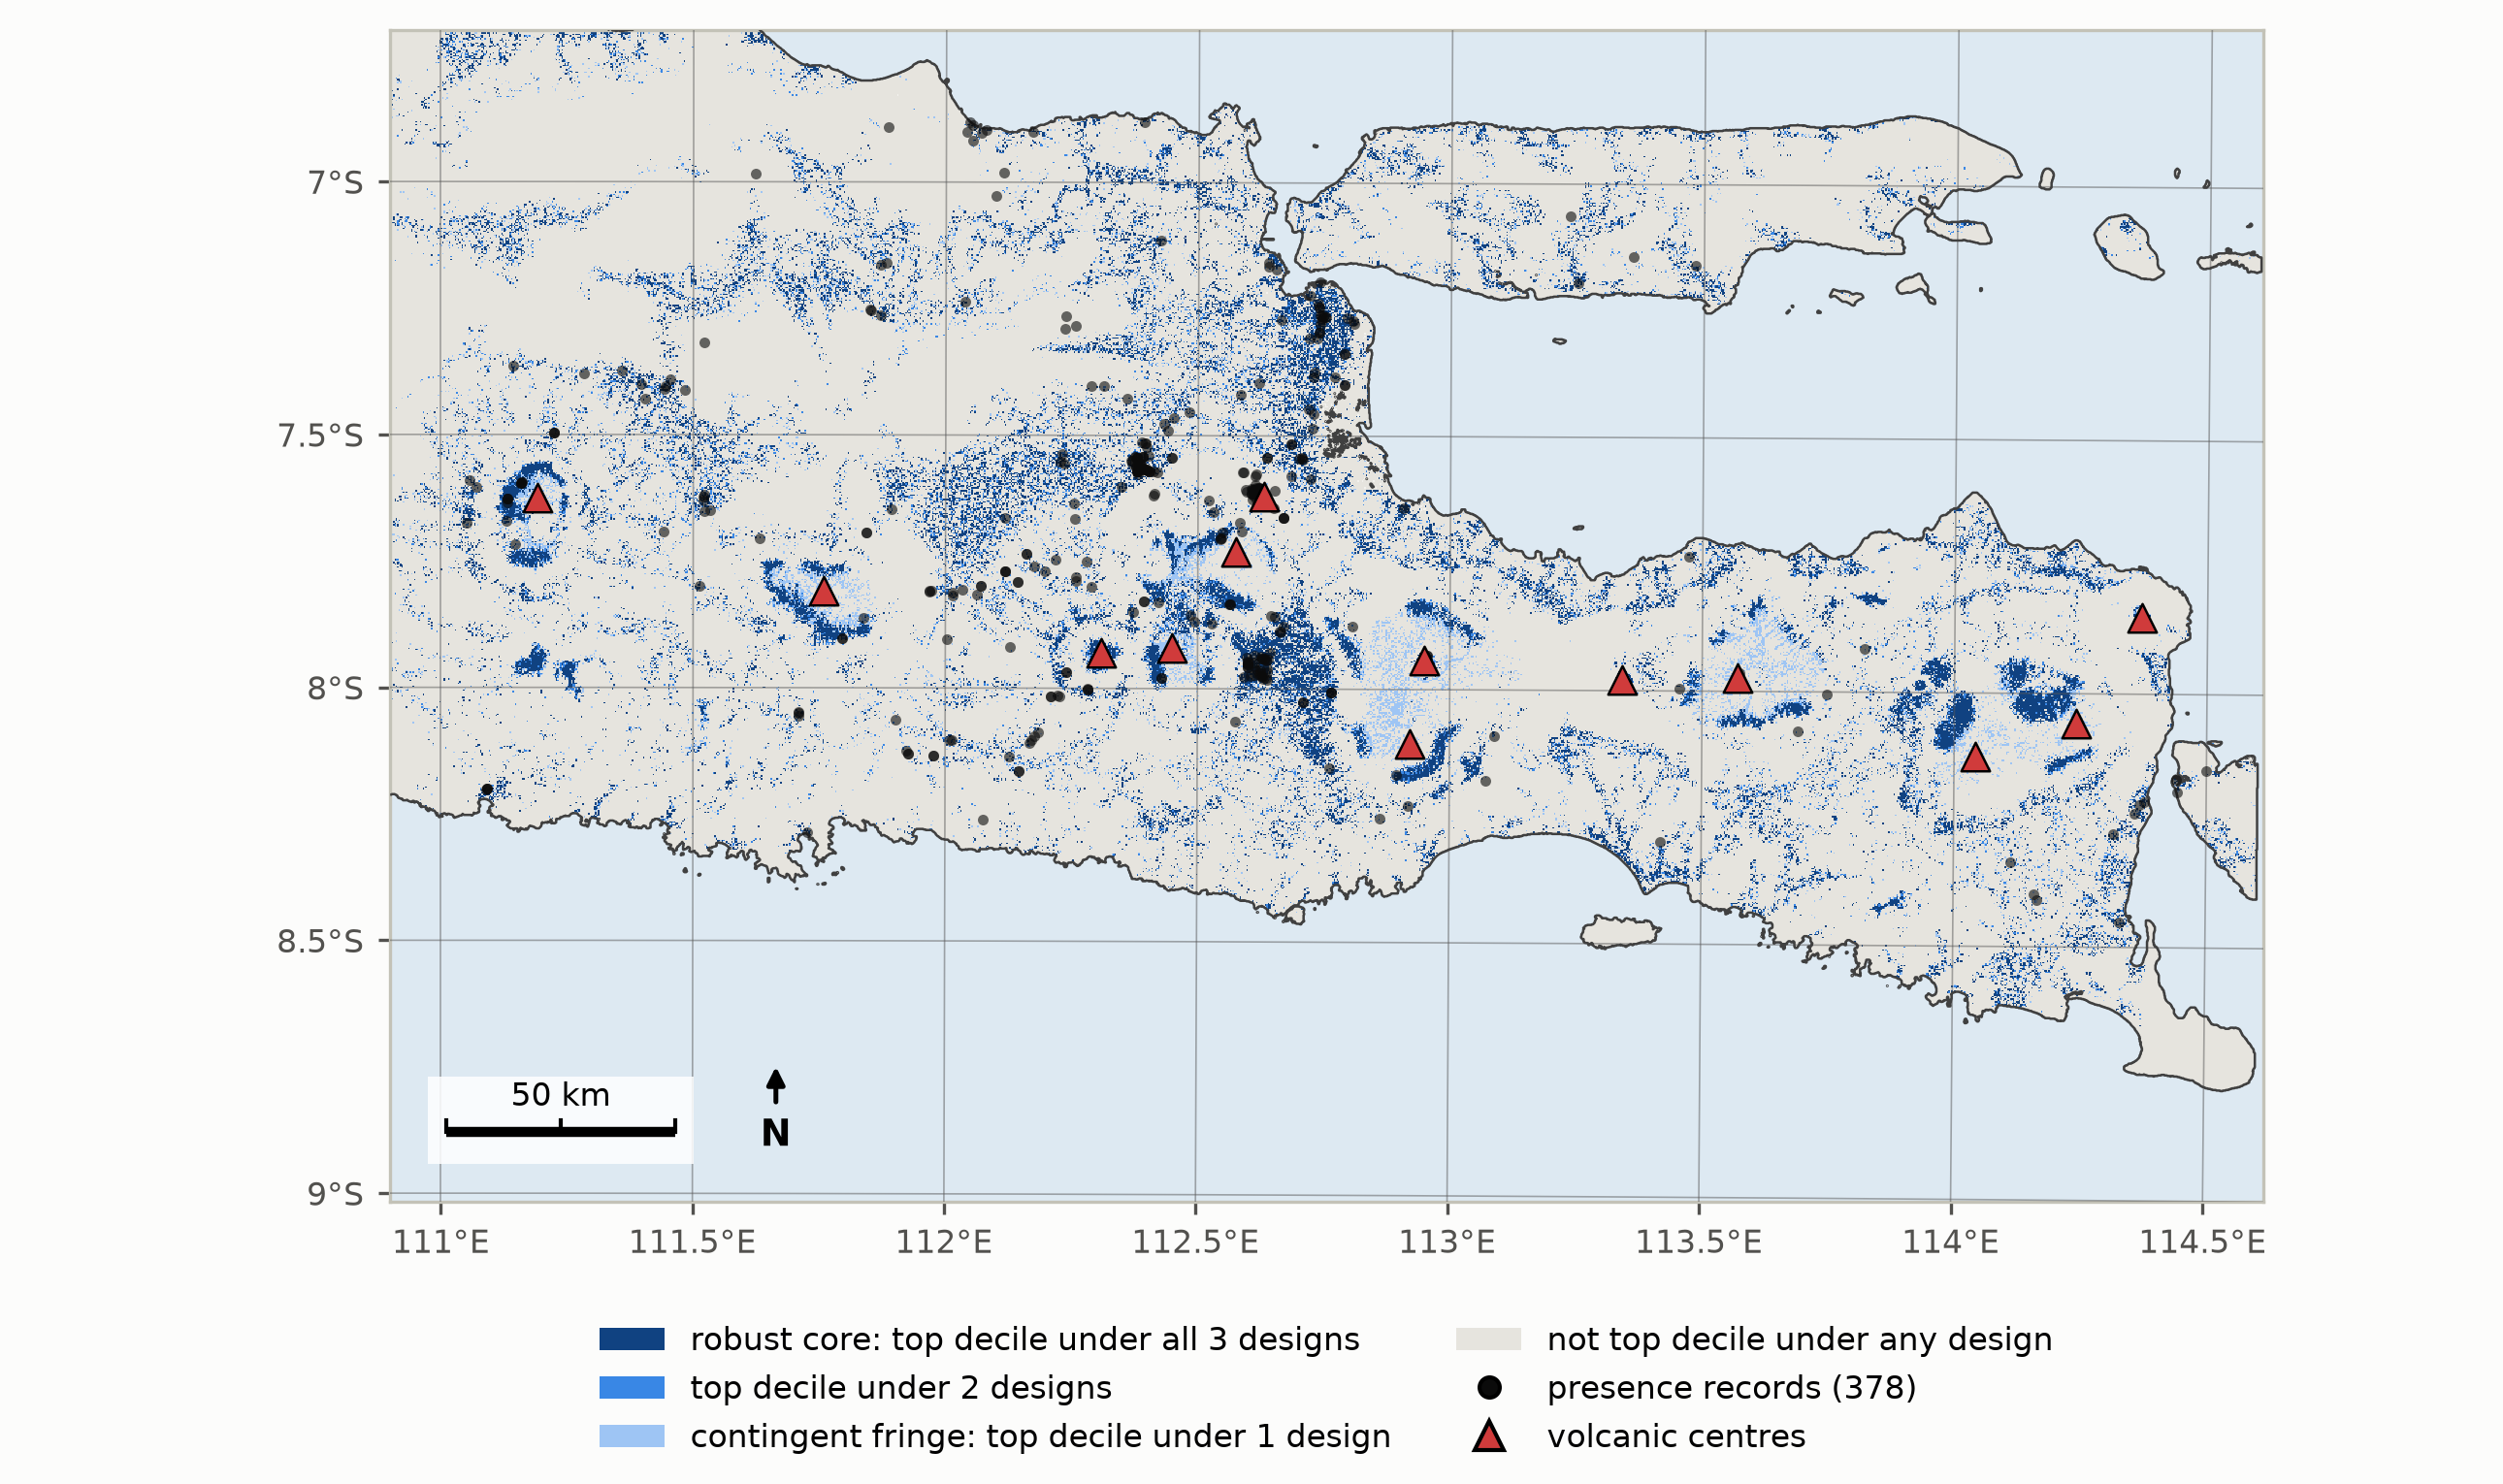
\includegraphics[width=\textwidth]{fig05_priority_map_v03.png}
\caption{Robust core and contingent fringe for XGBoost under a 10-seed ensemble, cells coloured by how many of the three background designs placed them in the top decile. The core concentrates on the accessible lowlands that hold most of the known records; the contingent fringe, where the background designs disagree, lies higher (median elevation 491~m for XGBoost and 1,107~m for MaxEnt).}
\label{fig:priority}
\end{figure}

\begin{figure}[h]
\centering
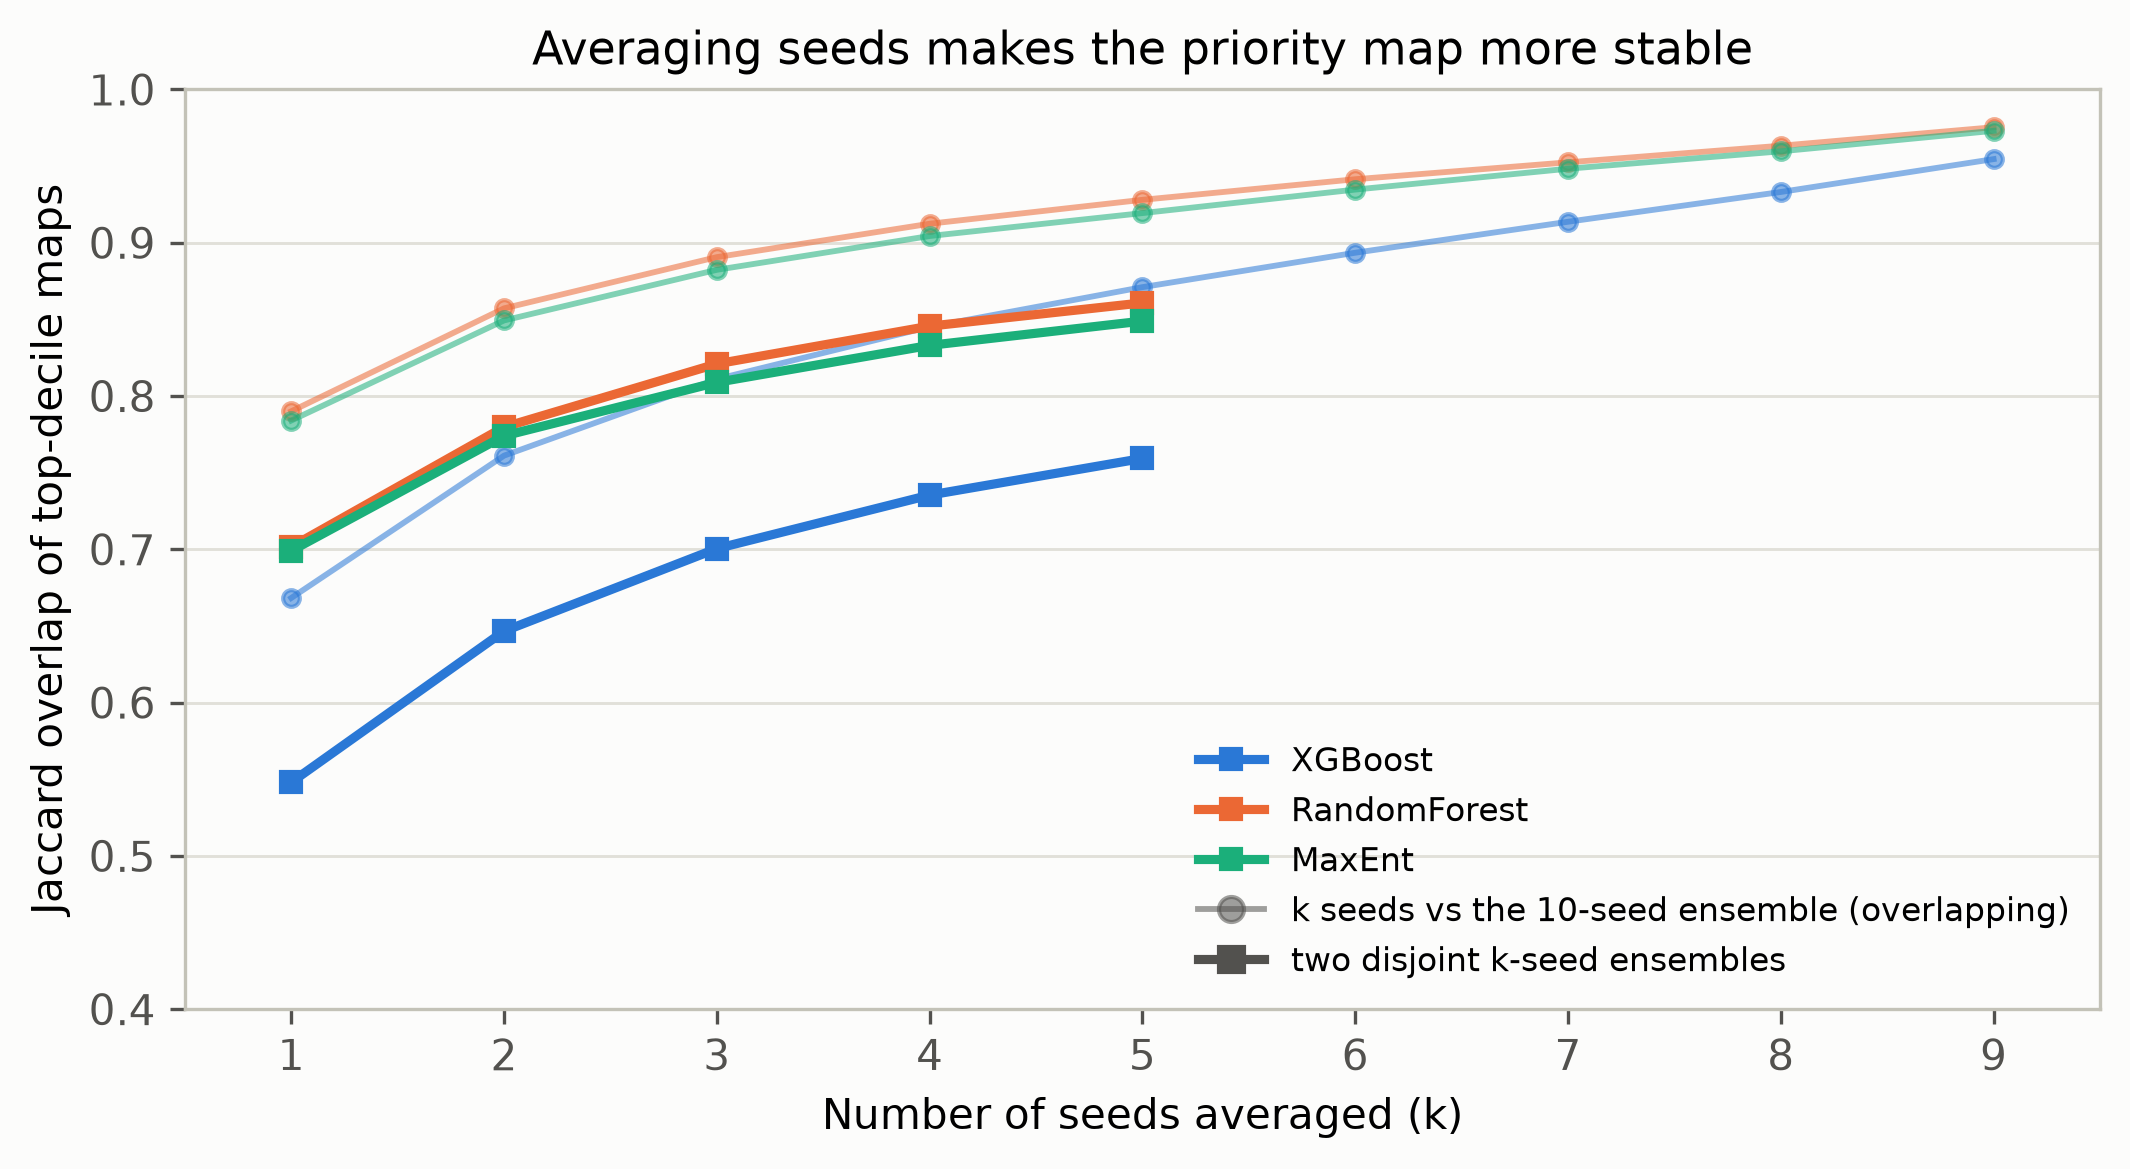
\includegraphics[width=0.8\textwidth]{fig06_seed_v03.png}
\caption{Agreement of top-decile priority maps as seeds are averaged, one colour per learner. Thin lines: an ensemble of $k$ seeds against the full 10-seed ensemble, which contains those seeds (E221). Thick lines: two ensembles of $k$ seeds that share no seed (E236; at most five seeds each from ten). The thick lines are the fair measure of stability.}
\label{fig:stabilisation}
\end{figure}

\subsection{Corrections to two volcanic diagnostics}
\label{sec:diagnostics}

\textbf{The volcano inventory.} The analysis code contained seven volcanic centres, whereas the canonical inventory includes 13 centres within the bounds of the study area (111--115$^\circ$E).
This correction to the inventory does not change the model AUCs, because \texttt{volcano\_dist} is not used as a training feature.
The result of Test 1 does change, however, because this test measures the correlation between predicted suitability and distance to volcanoes.
With 13 centres the Spearman value becomes $\rho = -0.281$, against $-0.243$ with seven centres.
Both correlations remain below the failure threshold of 0.5, so the verdict of Test 1 does not change.

% PI prose 2026-10-22 (passage 8D, first three sentences); closing rewritten by the PI 2026-11-10 (PI_PROSE_LOG_R3.md session 3).
\textbf{A correlation that is not consistent across seeds.} A single model instance gives a Spearman correlation of $-0.163$ for the same test.
However, repeating the analysis with five seeds on the same seven-volcano inventory gives $-0.243$ (E219).
This difference cannot be attributed to the seed alone.
E219 also changed the way the background is sampled, using a lattice rather than the continuous coordinates of the original pipeline.
Because both changed together, the effects of seed and sampling cannot be separated.
A single model instance is therefore not a sufficient basis for this diagnostic.
The values here use a five-seed ensemble; Table~\ref{tab:progression} presents the E007--E013 series from the original pipeline as the object under examination.

\subsection{Volcanic setting or elevation?}
\label{sec:elevation}

% PI prose 2026-10-21 (written in Indonesian, translated by Claude; log: PI_PROSE_LOG_R2.md, passage 2). Replaces the
% v0.2 terrain-matched control (E219 part C), which E235 supersedes.
This analysis tests whether the observed suitability pattern reflects a volcanic setting or simply the effect of elevation.
Distance to a volcanic centre (\texttt{volcano\_dist}) is not used as a training feature, so any pattern in the model's predictions that relates to a volcanic setting must come through the terrain variables the model uses.
Near land is defined as land within 20~km of a Quaternary volcanic centre, and far land as land 40~km or more from one; the analysis includes the 30 canonical volcanic centres, including those outside the map frame.
The comparison is made within each 200~m elevation band, using coarsened exact matching on slope, the terrain ruggedness index (TRI) and the topographic wetness index (TWI).
The analysis uses the stored 10-seed ensemble maps, without retraining any model.
Uncertainty is estimated with a spatial block bootstrap of 1,000 replicates; the decision threshold of 0.05 was set before the analysis, and the design was pre-registered in the public repository.
% PI prose 2026-10-21 (passage 3a).
The verdict labels follow the pre-registered rule: SPECIFIC if the 95\% CI excludes zero and the size of the difference is at least 0.05; NOT SPECIFIC if the whole 95\% CI lies between $-0.05$ and $+0.05$; and INCONCLUSIVE otherwise.

Above 1,000~m the study area contains about 3,435~km$^2$ of land, of which 97.5\% lies within 20~km of a Quaternary volcanic centre and only 0.4\% lies 40~km or more from one (Figure~\ref{fig:elevation}A).
Land far from Quaternary volcanic centres covers only about 15~km$^2$ at 1,000--1,200~m and none above 1,200~m.
In this study area, the effects of elevation and of proximity to a Quaternary volcanic centre cannot be adequately separated above about 1,000~m.
This study therefore does not attribute the pattern there specifically to either elevation or volcanic setting.
This limit of separability can shift between 800 and 1,200~m, depending on the minimum-area criterion used.

Below 1,000~m, the difference in suitability between land near and far from Quaternary volcanic centres is $+0.049$ for the random design (95\% CI $+0.024$ to $+0.077$), $+0.049$ for TGB and $+0.060$ for hybrid (95\% CI $+0.030$ to $+0.091$; Figure~\ref{fig:elevation}B).
Under the pre-registered rule, the hybrid result meets the criterion for SPECIFIC, but the summary across designs remains INCONCLUSIVE, because two of the three designs do not give a firm conclusion under that criterion.
% PI prose 2026-11-11 (session 4; log PI_PROSE_LOG_R3.md, session 4). Replaces the post hoc sentence from sessions 5-6,
% which was Claude's draft. F31: the quoted values are the random design's; F33: CI not repeated.
For the random design on XGBoost, the two pre-registered sensitivity definitions give smaller differences: $-0.002$ (NOT SPECIFIC) for near land within 10~km and far land beyond 30~km, and $+0.016$ (INCONCLUSIVE) with 15 and 30~km. The post hoc variants give $+0.005$ to $+0.067$, depending on the zone definitions and the matching procedure; additional matching on river distance lowers it to $+0.028$. The $+0.05$ sits exactly on the decision threshold, so the result gives no basis for claiming a direction below 1,000~m.
In the uplands (400--1,000~m), the far comparison land lies mostly in the Southern Mountains, an old volcanic arc of Eocene--Miocene age with karst landforms \citep{smyth2008}, so it would not be correct to call it non-volcanic.
In addition, the contingent fringe of the MaxEnt maps (Section~\ref{sec:prioritymaps}) has a median elevation of 1,107~m, above the limit of reliable separation; that pattern therefore cannot be interpreted specifically as either an elevation effect or a volcanic effect.
The limited power of the test also does not allow a firm conclusion about whether the disagreement between designs differs between near and far land.

\begin{figure}[t]
\centering
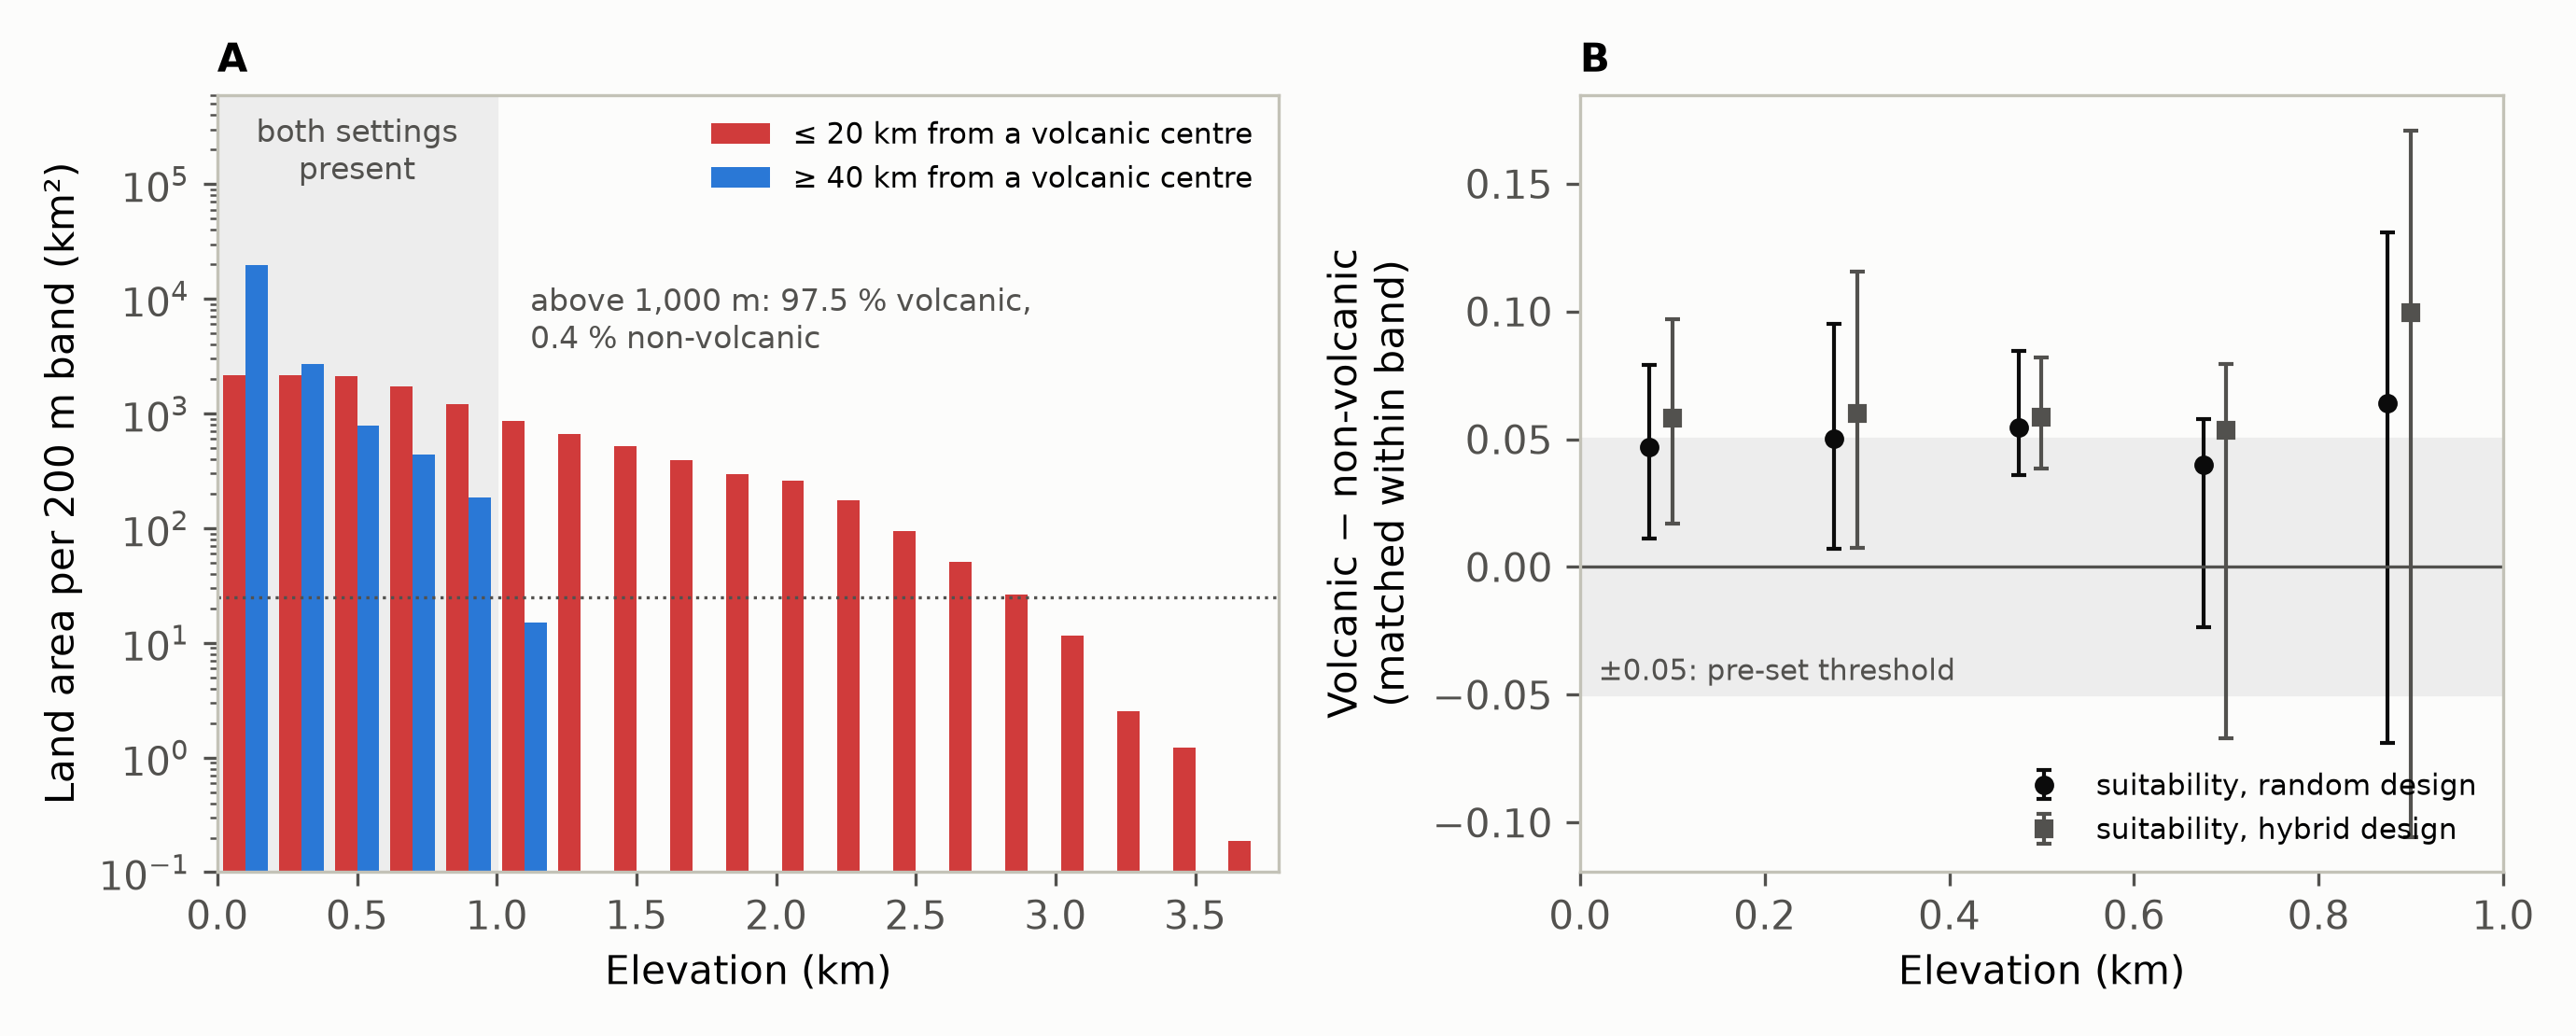
\includegraphics[width=\textwidth]{fig_e235_elevation_control_v03.png}
\caption{(A) Land area in each 200~m elevation band for land near ($\leq 20$~km) and far ($\geq 40$~km) from a Quaternary volcanic centre. (B) Difference in suitability between near and far land after matching on elevation, slope, TRI and TWI, with 95\% confidence intervals (XGBoost); the grey band marks the decision threshold of $\pm 0.05$.}
% Alt text (A4, approved 2026-10-21): Land area by elevation band and matched suitability differences
\label{fig:elevation}
\end{figure}

\subsection{What a suitability surface cannot show, and a quota design that failed}
\label{sec:withdrawal}

% PI prose 2026-10-22 (passage 8E, first sentence) and 2026-11-11 (sentences 2-3, session 4; log PI_PROSE_LOG_R3.md).
A suitability surface cannot distinguish the mechanisms that cause a site to go unobserved (Section~\ref{sec:taxonomy}).
Low predicted suitability near a volcano, on its own, cannot be taken as evidence that a settlement was buried.
The quota design also fails, both on World C, the regime of uneven survey effort between regions that motivated its development (true AUC difference $-0.2457$; Jaccard $-0.4688$; 0/30 pairs positive), and on World D, the balanced-truth regime most favourable to it ($-0.2027$ and $-0.2826$ respectively; 0/30).

% ============================================================================
\section{Discussion}
% ============================================================================

\subsection{Hold the evaluation background fixed}

The central methodological finding is that a background-design comparison is not identified unless the evaluation background is held fixed across the designs being compared, and that the artefact this produces is large enough to masquerade as a result.
How much real gain survives the correction depends on the presence data: the redesign gain is $-0.014$ AUC on the compiled records and about $+0.05$ on the cleaned sites (Section~\ref{sec:presence}).
The inflation that a common background removes does not depend on the data: it is $+0.037$ on the compiled records (60/60 cells) and $+0.041$ on the cleaned sites (54/60).
We are not the first to observe that background choice drives reported performance \citep{phillips2009, lobo2008, hijmans2012}; what we contribute is the mechanism (a selection criterion with no interior optimum, Section~\ref{sec:nooptimum}) and a direct quantification of the inflation it produces (for the hybrid design, all 240 synthetic runs and 60/60 and 54/60 real seed$\times$algorithm cells on the two presence sets).
The practical recommendation follows directly: \emph{report background designs on a common evaluation background, and state the evaluation availability domain of every metric}.
This is the accessible-area requirement of \citet{barve2011} applied to evaluation rather than to fitting: the domain over which a metric is computed is part of the metric, and a number reported without it cannot be compared with another.
We learned this from our own model.

\subsection{The archaeological content is in the background}

What makes a presence--background model archaeological, rather than a generic classifier run on coordinates, is not the label set.
It is the background design: a statement about where a survey could plausibly have detected a site had one been present.
That is what TGB and hybrid designs encode, and it is why they are archaeological choices rather than sampling conveniences.
The sharp corollary, which this paper exists to state, is that because the archaeological content lives in the background, and because the model was evaluated against that same background, the very thing that made the design archaeological is what contaminated its evaluation.

\subsection{A suitability surface is not a discovery map}

The output is a suitability surface with declared limits, not a map of where sites are.
Low suitability does not mean `buried' or `destroyed'; high suitability does not mean `a site is there' (Section~\ref{sec:taxonomy}).

\subsection{Implications for heritage management in East Java}

Under Indonesia's Cagar Budaya framework (UU 11/2010), surveys by the regional heritage preservation office (for East Java, Balai Pelestarian Kebudayaan Wilayah XI, until 2022 the Balai Pelestarian Cagar Budaya, BPCB) inform permitting and rescue prioritisation.
A suitability surface could in principle support that workflow, but only under two conditions this study makes explicit.
First, because priority maps turn over by $28$--$47\%$ between seeds (Section~\ref{sec:prioritymaps}), a single-seed map is not a defensible basis for a permit; the seed-ensemble protocol (at least seven seeds, with the agreement between disjoint ensembles reported) is a precondition for operational use.
Second, because the model reports suitability and not presence, the robust core ($1.9$--$5.6\times$ the density of records in the fringe on the compiled records, $2.5$--$8.5\times$ on the cleaned sites) is a prioritisation aid, not a prediction: it ranks where to look, not what will be found.

\subsection{The corrected protocol}

We summarise the protocol that follows from the above, which is the constructive contribution of this study:

\begin{enumerate}
  \item \textbf{Hold the evaluation background fixed} when comparing background designs; report own-background numbers only alongside common-background numbers.
  \item \textbf{Declare the availability domain} of every metric (background design, benchmark, selection rule).
  \item \textbf{Seed-ensemble priority maps} (at least seven seeds) and report the agreement between ensembles that share no seed; report a robust core and contingent fringe, never a single-seed map.
  \item \textbf{Do not let the selection criterion decide where to stop}: because it has no interior optimum, justify where to stop varying a background-design parameter on external grounds, not by the criterion's own maximum.
\end{enumerate}

\subsection{Limitations}
\label{sec:limitations}

\begin{enumerate}
  \item \textbf{Calibration gap between synthetic and real.} At a hard-negative share of 0.30 (the largest tried in E013) the selection criterion picks hybrid on real data but random on synthetic data, so the synthetic worlds do not reproduce the real-data selection behaviour there. This limits transferring the E222 conclusions back to the real case.
  \item \textbf{The truth-slope sign is regime-contingent}: negative on real data, positive on synthetic. We do not claim `hard negatives are always bad.'
  \item \textbf{Four synthetic regimes are not a universal result.} Across the four worlds (road-bias, misspecified, regional-bias, balanced-regional-truth; $n \approx 300$--$500$), no background design exceeded uniform on truth recovery by a meaningful margin (aggregate difference $\approx -0.0004$ AUC; in the two road-bias and misspecified surfaces TGB scored above random in 27/60 runs). This is not a refutation of target-group background in general \citep{phillips2009}; it is a result for the regimes and sample sizes tested.
  \item \textbf{A detection floor of $\sim +0.03$} at $n=378$: smaller effects are indeterminate, not absent (Section~\ref{sec:ci}). The cleaned subset has 161 sites, so its floor is larger; the interval reported for its redesign contrast is over seeds, not over sites.
  \item \textbf{The Boyce index is a direction check, not a selector.} It tracks the truth only loosely (median rank correlation $+0.50$ with map agreement and $+0.54$ with true AUC, E222), so we use it only to confirm direction.
  % PI prose 2026-10-21 (passage 3b); replaces the v0.2 "n = 2 in the non-volcanic arm" item.
  \item Above about 1,000~m (the limit shifts between 800 and 1,200~m, depending on the minimum area used), \textbf{elevation and proximity to a Quaternary volcanic centre cannot be adequately separated} in the study area; the model's prediction pattern there, including the high-elevation fringe in Figure~\ref{fig:priority}, therefore cannot be attributed specifically to either factor (Section~\ref{sec:elevation}).
  \item \textbf{The two-stage `suitable but absent' decomposition} is declared future work: it tests \emph{why} sites are absent, which requires site-level prediction, which this design does not support, and burial-depth data at survey resolution are not yet available.
  \item \textbf{External transfer beyond East Java is untested.}
  \item \textbf{The cleaned presence set is defined by our own rule} (Section~\ref{sec:presence}); a different rule could retain more or fewer records, and the compiled set remains the one on which the original ladder was run.
  \item \textbf{The cleaned set's contingent fringe holds only 5 sites under XGBoost, 15 under RandomForest and 5 under MaxEnt}, so its density ratios are reported as a direction, not as precise magnitudes.
\end{enumerate}

% ============================================================================
\section{Conclusions}
% ============================================================================

% Drafted by Claude from the PI's passages 8A, 6, 8E and 2 at the PI's request, 2026-10-22 (log: session 4, part 2).
In this study, the reported AUC of a presence--background model for East Java rose overall from 0.659 (E007) to 0.751 (E013, mean over seeds) across seven experiments, and the rise was attributed to increasingly realistic background designs.
Scored on a common evaluation background, that rise is not reproduced on the 378 compiled records: redesigning the background contributes $-0.014$ AUC and adding distance to rivers contributes $+0.042$, and the last design, the hybrid, scores higher only when it is evaluated on its own background points.
Whether a real gain remains depends on the presence data. On 161 cleaned sites the same redesign contributes $+0.051$ AUC [$+0.039$, $+0.063$] over ten seeds, positive in 29 of 30 cells, and two disjoint halves of five seeds give $+0.0505$ and $+0.0516$; own-background evaluation still overstates that gain by about $+0.05$. The earlier target-group designs are not reproduced on either set.
Only a common evaluation background shows how much of the reported gain is real.
The criterion used to choose a design, AUC on the design's own background, has no optimum inside the range tested, so it gives no indication of when to stop adding hard negatives.
A suitability surface also cannot distinguish the reasons a site goes unobserved, so low predicted suitability near volcanoes is not evidence of buried settlement; and above about 1,000~m, elevation and proximity to a Quaternary volcanic centre cannot be adequately separated in East Java.

The contribution of this study is therefore a protocol, not a new prediction of site locations.
Background designs should be compared on a fixed evaluation background, the availability domain of every metric should be stated, and priority maps should be averaged over at least seven seeds, with the agreement between ensembles that share no seed reported.
We applied these checks to our own earlier analyses, where they changed the conclusion; they need no new data and can be applied to other presence--background comparisons.

% ============================================================================
\section*{Supplementary Materials}
% ============================================================================

% Mechanical 2026-10-21: v0.3 supplement file name, second build script, items S7-S8 (PI may reword the two items).
Supplied as a single document, \texttt{supplementary\_tables\_v0.3.pdf}. Every table in it is generated directly from the raw result files by \texttt{build\_supplement.py} and \texttt{build\_e235\_tables.py} (included in the code repository); no value is retyped.

\begin{itemize}
  \item \textbf{Table S1:} Seed stability --- XGBoost and RandomForest AUC and TSS across the 20 alternate seeds for E013.
  \item \textbf{Table S2:} Block-size sensitivity --- spatial CV at $\sim$40, $\sim$50 and $\sim$60 km, with 95\% intervals.
  \item \textbf{Table S3:} E217 common-background benchmark --- every design $\times$ feature set $\times$ algorithm, scored on its own background and on a common background.
  \item \textbf{Table S4:} E218 own- versus common-background matrix --- three training designs against four evaluation backgrounds.
  \item \textbf{Table S5:} E222 synthetic worlds --- reported against true AUC by background configuration and algorithm.
  \item \textbf{Table S6:} Per-experiment design matrix for E217--E224 (extends Table~\ref{tab:inclusion}), including which experiments used \texttt{road\_dist} as a feature.
  \item \textbf{Table S7:} E235 elevation bands --- land near and far from Quaternary volcanic centres in each 200~m band, and the matched near $-$ far differences (Section~\ref{sec:elevation}).
  \item \textbf{Table S8:} E235 pooled differences --- by zone definition and algorithm, with the pre-registered verdicts.
  \item \textbf{Table S9:} E236 --- the same real-data quantities on the compiled records and on the cleaned presences (Section~\ref{sec:presence}).
\end{itemize}

% ============================================================================
\section*{Acknowledgements}
% ============================================================================

The authors thank the editor and the anonymous reviewers for comments that substantially improved this paper.

\subsection*{Funding}
This research received no external funding.

\subsection*{Competing Interests}
The authors have no competing interests to declare.

\subsection*{Authors' Contributions}
M.A.\ conceived the study and its design, directed and checked the analyses (implemented with AI assistance, as declared below), curated the data, and prepared the manuscript.
G.F.G.\ contributed to methodology refinement, code review, and manuscript editing.
Both authors read and approved the final manuscript.

\subsection*{Data Availability}

\textbf{Archaeological site data:} the compiled East Java site dataset is in the repository at \texttt{data/processed/east\_java\_sites.geojson} (378 with valid covariates in bounds: 279 from OpenStreetMap, 85 from lists in the Indonesian and English Wikipedia, 14 from Wikidata). Licences: OpenStreetMap (ODbL), Wikipedia (CC BY-SA), Wikidata (CC0). The cleaned subset of 161 sites (Section~\ref{sec:presence}) is derived from this file by \texttt{clean\_sites.py} in the E236 folder.

\textbf{Environmental covariates:} Copernicus GLO-30 DEM and derived layers from the Copernicus Programme (ESA), \url{https://dataspace.copernicus.eu/}. OpenStreetMap road and river data, \url{https://openstreetmap.org} (ODbL).

\textbf{Code:} all source code, including E217--E224, E235, E236 and the verification script, is at \url{https://github.com/neimasilk/volcarch-repo} (MIT licence).\newline The G1 verification script is \texttt{verify\_headline\_numbers.py}.\newline Python dependencies are pinned in \texttt{requirements\_submission\_lock.txt}.

\textbf{Interactive dashboard:} \url{https://volcarch-dashboard.streamlit.app}.

\subsection*{Declaration of AI Use}

We used Claude (Anthropic) throughout this study.
It wrote and debugged the analysis code, produced the figures, drafted the designs of the experiments described in Section~\ref{sec:refutation}, checked the references against Crossref and the cited papers, and re-derived every reported number from the raw result files.
It also helped with the text.
The earlier drafts of the Methods, Results and Discussion were generated with Claude from our analyses and notes, and were then revised by us.
In this version, new passages were written by the first author in Indonesian and translated into English with Claude, and the restatements of the abstract, the conclusions and the affected parts of the Results and Discussion were drafted with Claude at the first author's request and then checked and approved by the author.
The research questions, the decisions about what to test and what to claim, and the interpretation are ours.
We checked every statement and number against the results and take full responsibility for the content.

% Generated by build_jcaa_bibliography.py from references.bib -- do not edit by hand.
\begingroup\raggedright
\begin{thebibliography}{30}

\bibitem[Allouche, Tsoar \& Kadmon(2006)]{allouche2006}
Allouche, O, Tsoar, A and Kadmon, R. 2006. Assessing the accuracy of species distribution models: prevalence, kappa and the true skill statistic (TSS). \textit{Journal of Applied Ecology}, 43(6): 1223–1232. DOI: 10.1111/j.1365-2664.2006.01214.x

\bibitem[Ara{\'u}jo \& Guisan(2006)]{araujo2006}
Ara{\'u}jo, MB and Guisan, A. 2006. Five (or so) challenges for species distribution modelling. \textit{Journal of Biogeography}, 33(10): 1677–1688. DOI: 10.1111/j.1365-2699.2006.01584.x

\bibitem[Banks et~al.(2006)]{banks2006}
Banks, WE, d'Errico, F, Dibble, HL, Krishtalka, L, West, D, Olszewski, DI, Peterson, AT, Anderson, DG, Gillam, JC, Montet-White, A, Crucifix, M, Marean, CW, S{\'a}nchez-Go{\~n}i, M-F, Wohlfarth, B and Vanhaeren, M. 2006. Eco-cultural niche modeling: new tools for reconstructing the geography and ecology of past human populations. \textit{PaleoAnthropology}, 68–83.

\bibitem[Barbet-Massin et~al.(2012)]{barbet2012}
Barbet-Massin, M, Jiguet, F, Albert, CH and Thuiller, W. 2012. Selecting pseudo-absences for species distribution models: how, where and how many? \textit{Methods in Ecology and Evolution}, 3(2): 327–338. DOI: 10.1111/j.2041-210X.2011.00172.x

\bibitem[Barve et~al.(2011)]{barve2011}
Barve, N, Barve, V, Jim{\'e}nez-Valverde, A, Lira-Noriega, A, Maher, SP, Peterson, AT, Sober{\'o}n, J and Villalobos, F. 2011. The crucial role of the accessible area in ecological niche modeling and species distribution modeling. \textit{Ecological Modelling}, 222(11): 1810–1819. DOI: 10.1016/j.ecolmodel.2011.02.011

\bibitem[Breiman(2001)]{breiman2001}
Breiman, L. 2001. Random forests. \textit{Machine Learning}, 45(1): 5–32. DOI: 10.1023/A:1010933404324

\bibitem[Castiello \& Tonini(2021)]{castiello2021}
Castiello, ME and Tonini, M. 2021. An explorative application of Random Forest algorithm for archaeological predictive modeling. A Swiss case study. \textit{Journal of Computer Applications in Archaeology}, 4(1): 110–125. DOI: 10.5334/jcaa.71

\bibitem[Chen \& Guestrin(2016)]{chen2016}
Chen, T and Guestrin, C. 2016. XGBoost: a scalable tree boosting system. In: \textit{Proceedings of the 22nd ACM SIGKDD International Conference on Knowledge Discovery and Data Mining}. ACM, pp. 785–794. DOI: 10.1145/2939672.2939785

\bibitem[Comer et~al.(2023)]{comer2023}
Comer, JA, Comer, DC, Dumitru, IA, Priebe, CE and Patsolic, JL. 2023. Sampling methods for archaeological predictive modeling: spatial autocorrelation and model performance. \textit{Journal of Archaeological Science: Reports}, 48: Article 103824. DOI: 10.1016/j.jasrep.2022.103824

\bibitem[Elith et~al.(2006)]{elith2006}
Elith, J, Graham, CH, Anderson, RP, Dud{\'{\i}}k, M, Ferrier, S, Guisan, A, Hijmans, RJ, Huettmann, F, Leathwick, JR, Lehmann, A, Li, J, Lohmann, LG, Loiselle, BA, Manion, G, Moritz, C, Nakamura, M, Nakazawa, Y, Overton, JMcC, Peterson, AT, Phillips, SJ, Richardson, K, Scachetti-Pereira, R, Schapire, RE, Sober{\'o}n, J, Williams, S, Wisz, MS and Zimmermann, NE. 2006. Novel methods improve prediction of species' distributions from occurrence data. \textit{Ecography}, 29(2): 129–151. DOI: 10.1111/j.2006.0906-7590.04596.x

\bibitem[Franklin(2009)]{franklin2009}
Franklin, J. 2009. \textit{Mapping Species Distributions: Spatial Inference and Prediction.} Cambridge: Cambridge University Press. DOI: 10.1017/CBO9780511810602

\bibitem[Guillera-Arroita et~al.(2015)]{guillera2015}
Guillera-Arroita, G, Lahoz-Monfort, JJ, Elith, J, Gordon, A, Kujala, H, Lentini, PE, McCarthy, MA, Tingley, R and Wintle, BA. 2015. Is my species distribution model fit for purpose? Matching data and models to applications. \textit{Global Ecology and Biogeography}, 24(3): 276–292. DOI: 10.1111/geb.12268

\bibitem[Hijmans(2012)]{hijmans2012}
Hijmans, RJ. 2012. Cross-validation of species distribution models: removing spatial sorting bias and calibration with a null model. \textit{Ecology}, 93(3): 679–688. DOI: 10.1890/11-0826.1

\bibitem[Howey, Palace \& McMichael(2016)]{howey2016}
Howey, MCL, Palace, MW and McMichael, CH. 2016. Geospatial modeling approach to monument construction using Michigan from A.D. 1000--1600 as a case study. \textit{Proceedings of the National Academy of Sciences}, 113(27): 7443–7448. DOI: 10.1073/pnas.1603450113

\bibitem[Kvamme(2006)]{kvamme2006}
Kvamme, KL. 2006. There and back again: revisiting archaeological locational modeling. In: Mehrer, MW and Wescott, KL (eds.) \textit{GIS and Archaeological Site Location Modeling}. Boca Raton: Taylor \& Francis, pp. 3–38. DOI: 10.1201/9780203563359.sec1

\bibitem[Lobo, Jim{\'e}nez-Valverde \& Hortal(2010)]{lobo2010}
Lobo, JM, Jim{\'e}nez-Valverde, A and Hortal, J. 2010. The uncertain nature of absences and their importance in species distribution modelling. \textit{Ecography}, 33(1): 103–114. DOI: 10.1111/j.1600-0587.2009.06039.x

\bibitem[Lobo, Jim{\'e}nez-Valverde \& Real(2008)]{lobo2008}
Lobo, JM, Jim{\'e}nez-Valverde, A and Real, R. 2008. AUC: a misleading measure of the performance of predictive distribution models. \textit{Global Ecology and Biogeography}, 17(2): 145–151. DOI: 10.1111/j.1466-8238.2007.00358.x

\bibitem[Noviello et~al.(2018)]{noviello2018}
Noviello, M, Cafarelli, B, Calculli, C, Sarris, A and Mairota, P. 2018. Investigating the distribution of archaeological sites: multiparametric vs probability models and potentials for remote sensing data. \textit{Applied Geography}, 95: 34–44. DOI: 10.1016/j.apgeog.2018.04.005

\bibitem[Phillips, Anderson \& Schapire(2006)]{phillips2006}
Phillips, SJ, Anderson, RP and Schapire, RE. 2006. Maximum entropy modeling of species geographic distributions. \textit{Ecological Modelling}, 190(3–4): 231–259. DOI: 10.1016/j.ecolmodel.2005.03.026

\bibitem[Phillips et~al.(2009)]{phillips2009}
Phillips, SJ, Dud{\'{\i}}k, M, Elith, J, Graham, CH, Lehmann, A, Leathwick, J and Ferrier, S. 2009. Sample selection bias and presence-only distribution models: implications for background and pseudo-absence data. \textit{Ecological Applications}, 19(1): 181–197. DOI: 10.1890/07-2153.1

\bibitem[Radosavljevic \& Anderson(2014)]{radosavljevic2014}
Radosavljevic, A and Anderson, RP. 2014. Making better Maxent models of species distributions: complexity, overfitting and evaluation. \textit{Journal of Biogeography}, 41(4): 629–643. DOI: 10.1111/jbi.12227

\bibitem[Roberts et~al.(2017)]{roberts2017}
Roberts, DR, Bahn, V, Ciuti, S, Boyce, MS, Elith, J, Guillera-Arroita, G, Hauenstein, S, Lahoz-Monfort, JJ, Schr{\"o}der, B, Thuiller, W, Warton, DI, Wintle, BA, Hartig, F and Dormann, CF. 2017. Cross-validation strategies for data with temporal, spatial, hierarchical, or phylogenetic structure. \textit{Ecography}, 40(8): 913–929. DOI: 10.1111/ecog.02881

\bibitem[Senay, Worner \& Ikeda(2013)]{senay2013}
Senay, SD, Worner, SP and Ikeda, T. 2013. Novel three-step pseudo-absence selection technique for improved species distribution modelling. \textit{PLOS ONE}, 8(8): Article e71218. DOI: 10.1371/journal.pone.0071218

\bibitem[Smyth, Hall \& Nichols(2008)]{smyth2008}
Smyth, HR, Hall, R and Nichols, GJ. 2008. Cenozoic volcanic arc history of East Java, Indonesia: the stratigraphic record of eruptions on an active continental margin. In: Draut, AE, Clift, PD and Scholl, DW (eds.) \textit{Formation and Applications of the Sedimentary Record in Arc Collision Zones}. Boulder, CO: Geological Society of America, pp. 199–222. DOI: 10.1130/2008.2436(10)

\bibitem[Valavi et~al.(2019)]{valavi2019}
Valavi, R, Elith, J, Lahoz-Monfort, JJ and Guillera-Arroita, G. 2019. blockCV: an R package for generating spatially or environmentally separated folds for k-fold cross-validation of species distribution models. \textit{Methods in Ecology and Evolution}, 10(2): 225–232. DOI: 10.1111/2041-210X.13107

\bibitem[Verhagen \& Whitley(2012)]{verhagen2012}
Verhagen, P and Whitley, TG. 2012. Integrating archaeological theory and predictive modeling: a live report from the scene. \textit{Journal of Archaeological Method and Theory}, 19(1): 49–100. DOI: 10.1007/s10816-011-9102-7

\bibitem[Wang, Shi \& Oguchi(2023)]{wang2023}
Wang, Y, Shi, X and Oguchi, T. 2023. Archaeological predictive modeling using machine learning and statistical methods for Japan and China. \textit{ISPRS International Journal of Geo-Information}, 12(6): Article 238. DOI: 10.3390/ijgi12060238

\bibitem[Warren \& Seifert(2011)]{warren2011}
Warren, DL and Seifert, SN. 2011. Ecological niche modeling in Maxent: the importance of model complexity and the performance of model selection criteria. \textit{Ecological Applications}, 21(2): 335–342. DOI: 10.1890/10-1171.1

\bibitem[Wisz \& Guisan(2009)]{wisz2009}
Wisz, MS and Guisan, A. 2009. Do pseudo-absence selection strategies influence species distribution models and their predictions? An information-theoretic approach based on simulated data. \textit{BMC Ecology}, 9: Article 8. DOI: 10.1186/1472-6785-9-8

\bibitem[Yaworsky et~al.(2020)]{yaworsky2020}
Yaworsky, PM, Vernon, KB, Spangler, JD, Brewer, SC and Codding, BF. 2020. Advancing predictive modeling in archaeology: an evaluation of regression and machine learning methods on the Grand Staircase-Escalante National Monument. \textit{PLOS ONE}, 15(10): Article e0239424. DOI: 10.1371/journal.pone.0239424

\end{thebibliography}
\endgroup


\section*{Figure Alt Text}
\begin{itemize}
  \item Figure 1: Relief map of East Java with sites and volcanoes.
  \item Figure 2: Bar charts of AUC and TSS across seven experiments.
  \item Figure 3: Two panels comparing own-background and common-background model scores.
  \item Figure 4: Reported versus true performance as hard negatives increase.
  \item Figure 5: Map of East Java coloured by agreement between designs.
  \item Figure 6: Map agreement rising with the number of seeds averaged.
  \item Figure 7: Land area by elevation band and matched suitability differences.
\end{itemize}

\end{document}
